\noindent {\bf Chapter Editors:}~Simon Knapen, Jessie Shelton
\\


\noindent {\bf Additional Contributors:}~Michael Adersberger, James Beacham, Malte Buschmann, Cari Cesarotti, Marat Freytsis, Gregor Kasieczka, Joachim Kopp, Matt LeBlanc, Dylan Linthorne,  Sascha Mehlhase, Siddharth Mishra-Sharma, Matt Reece, Jakub Scholtz, Pedro Schwaller, Daniel Stolarski, Yuhsin Tsai

\section{Introduction: The anatomy of a dark shower}
\label{sec:darkshowerintro}
\JS{referencing is only preliminary}

Hidden sectors are increasingly common features in many models that address mysteries of particle physics such as the hierarchy problem, the origins of dark matter, baryogenesis, and neutrino masses.  In more generality, hidden sectors or ``hidden valleys'' are a generic possibility for physics beyond the Standard Model \cite{Strassler:2006im,Han:2007ae}.  Given the complexity of the Standard Model, such hidden sectors may very well have rich dynamics of their own, with strong implications for their phenomenology \cite{Strassler:2006ri,Strassler:2006qa,Strassler:2008bv,Strassler:2008fv,Juknevich:2009ji}. 
The main LHC signatures predicted by such hidden valley models are characterized by an injection of a relatively large amount of energy into a hidden sector, which is then shared among a large number of relatively soft particles \cite{Strassler:2008bv}. We will refer to this class of signatures, where rich dynamics internal to the hidden sector yields a high multiplicity of dark states, as ``dark showers''.
Given that the particles emerging at the end of this process are necessarily both (relatively) light and secluded from the SM, their lifetimes can easily become long, thus giving rise to displaced signatures at the LHC.

LLPs are especially generic predictions of hidden valleys with confining gauge groups, similar to QCD in the SM
\cite{Strassler:2006im}. It is worth noting that QCD already provides many familiar examples of
long-lived particles, realizing macroscopic lifetimes through a hierarchy of scales ($\Lambda_{QCD}/m_W$) combined with
approximately preserved symmetries ($K_L$, $B$ and $D$ hadrons) or
restricted phase space ($n$). QCD also provides numerous
examples of particles that have a hierarchy of lifetimes: for
instance, charged pions experience a slow decay through a very off-shell $W$ boson, 
while neutral pions can decay much faster through its anomalous
coupling to photons.  The neutral pion lifetime is thus
orders of magnitude shorter than the lifetime for charged pions.  Both
long-lived species and a hierarchy of lifetimes between species are
generic predictions and nearly unavoidable consequences of confining
theories which produce dark showers.  However LLPs with a hierarchy of
lifetimes also arise naturally in non-confining hidden sectors,
especially in theories with multiple species.  A familiar example from
the literature is theories with dark photons.  Here small kinetic
mixing can make the dark photon long-lived \cite{} \JS{refs needed}\SK{meh, obvious no?}, but the
simple well-motivated extension of the model by a dark Higgs boson
introduces additional dark species,  production mechanisms for dark states that are independent of the small coupling controlling the macroscopic lifetime, and naturally yields
high-multiplicity events featuring particles with a hierarchy of
lifetimes \cite{Schabinger:2005ei,Chan:2011aa, Curtin:2014cca}.



More generally, a dark shower topology can be broken down in three components (see Fig.~\ref{fig:showerdiagram}), each of which allows for a large degree of variation between models:
\begin{enumerate}
\item \textbf{Production.} A dark shower event begins with the production of one or more heavy states which decay into the dark sector. These heavy states could be part of the SM, most notably the Higgs boson, or could be a new particle from the menu of BSM states we have become accustomed to ($Z'$s, color triplets/octets, electroweak doublets/triplets etc). In some cases the production mechanism provides an important trigger handle (e.g. $VH$  production for the Higgs), but this is not universally the case (e.g. $Z'$ production). The options for production are laid out in Sec.~\ref{sec:darkshowerprod}.

\item \textbf{Showering and hadronization.} If the dark sector contains an asymptotically free gauge group, the originally produced particles will shower and possibly hadronize within the dark sector. This yields a final state with a potentially large number of dark states, similarly to how quarks and gluons undergo showering and hadronization to yield a jet of hadrons. The shape of the shower and the $p_T$ spectrum depends on the coupling of the dark gauge group: the shower may be pencil-like, as in QCD, completely spherically symmetric, or something in between. Alternatively, it is possible that the hidden sector does not contain a gauge sector but instead features a perturbative cascade decay over a large number of states. Indeed, in certain cases the perturbative picture is dual to the strongly coupled showers.
In general showering and hadronization  is the  source of greatest uncertainty on the theory side; the current status and some new results are discussed in Sec.~\ref{sec:darkshowershower}. 
   
\item \textbf{Decay.} After the dark degrees of freedom hadronize, or reach the bottom of the cascade in perturbative models, they can decay back to the SM. The decay may occur through the same (off-shell) portal as the production, but this is not essential, and one may expect multiple species with a range of lifetimes. The specifics of the decay step (e.g. muon multiplicity) are particularly important if there is no good trigger handle from the production topology. Decays are frequently interconnected with  showering and especially hadronization, however, and it is not tractable to enumerate all possibilities without making simplifying assumptions and/or inserting additional theory prejudice. For this reason it is often useful to focus on the species with the largest multiplicity and/or shortest (macroscopic) lifetime; this frequently provides a reasonable guide to the overall signatures, just as one may obtain a reasonable $O(1)$ picture of QCD jets by considering only its pions.  We survey a (non-exhaustive list) of popular decay portals in Sec.~\ref{sec:darkshowerdk}.
 
\begin{figure}[t]\centering
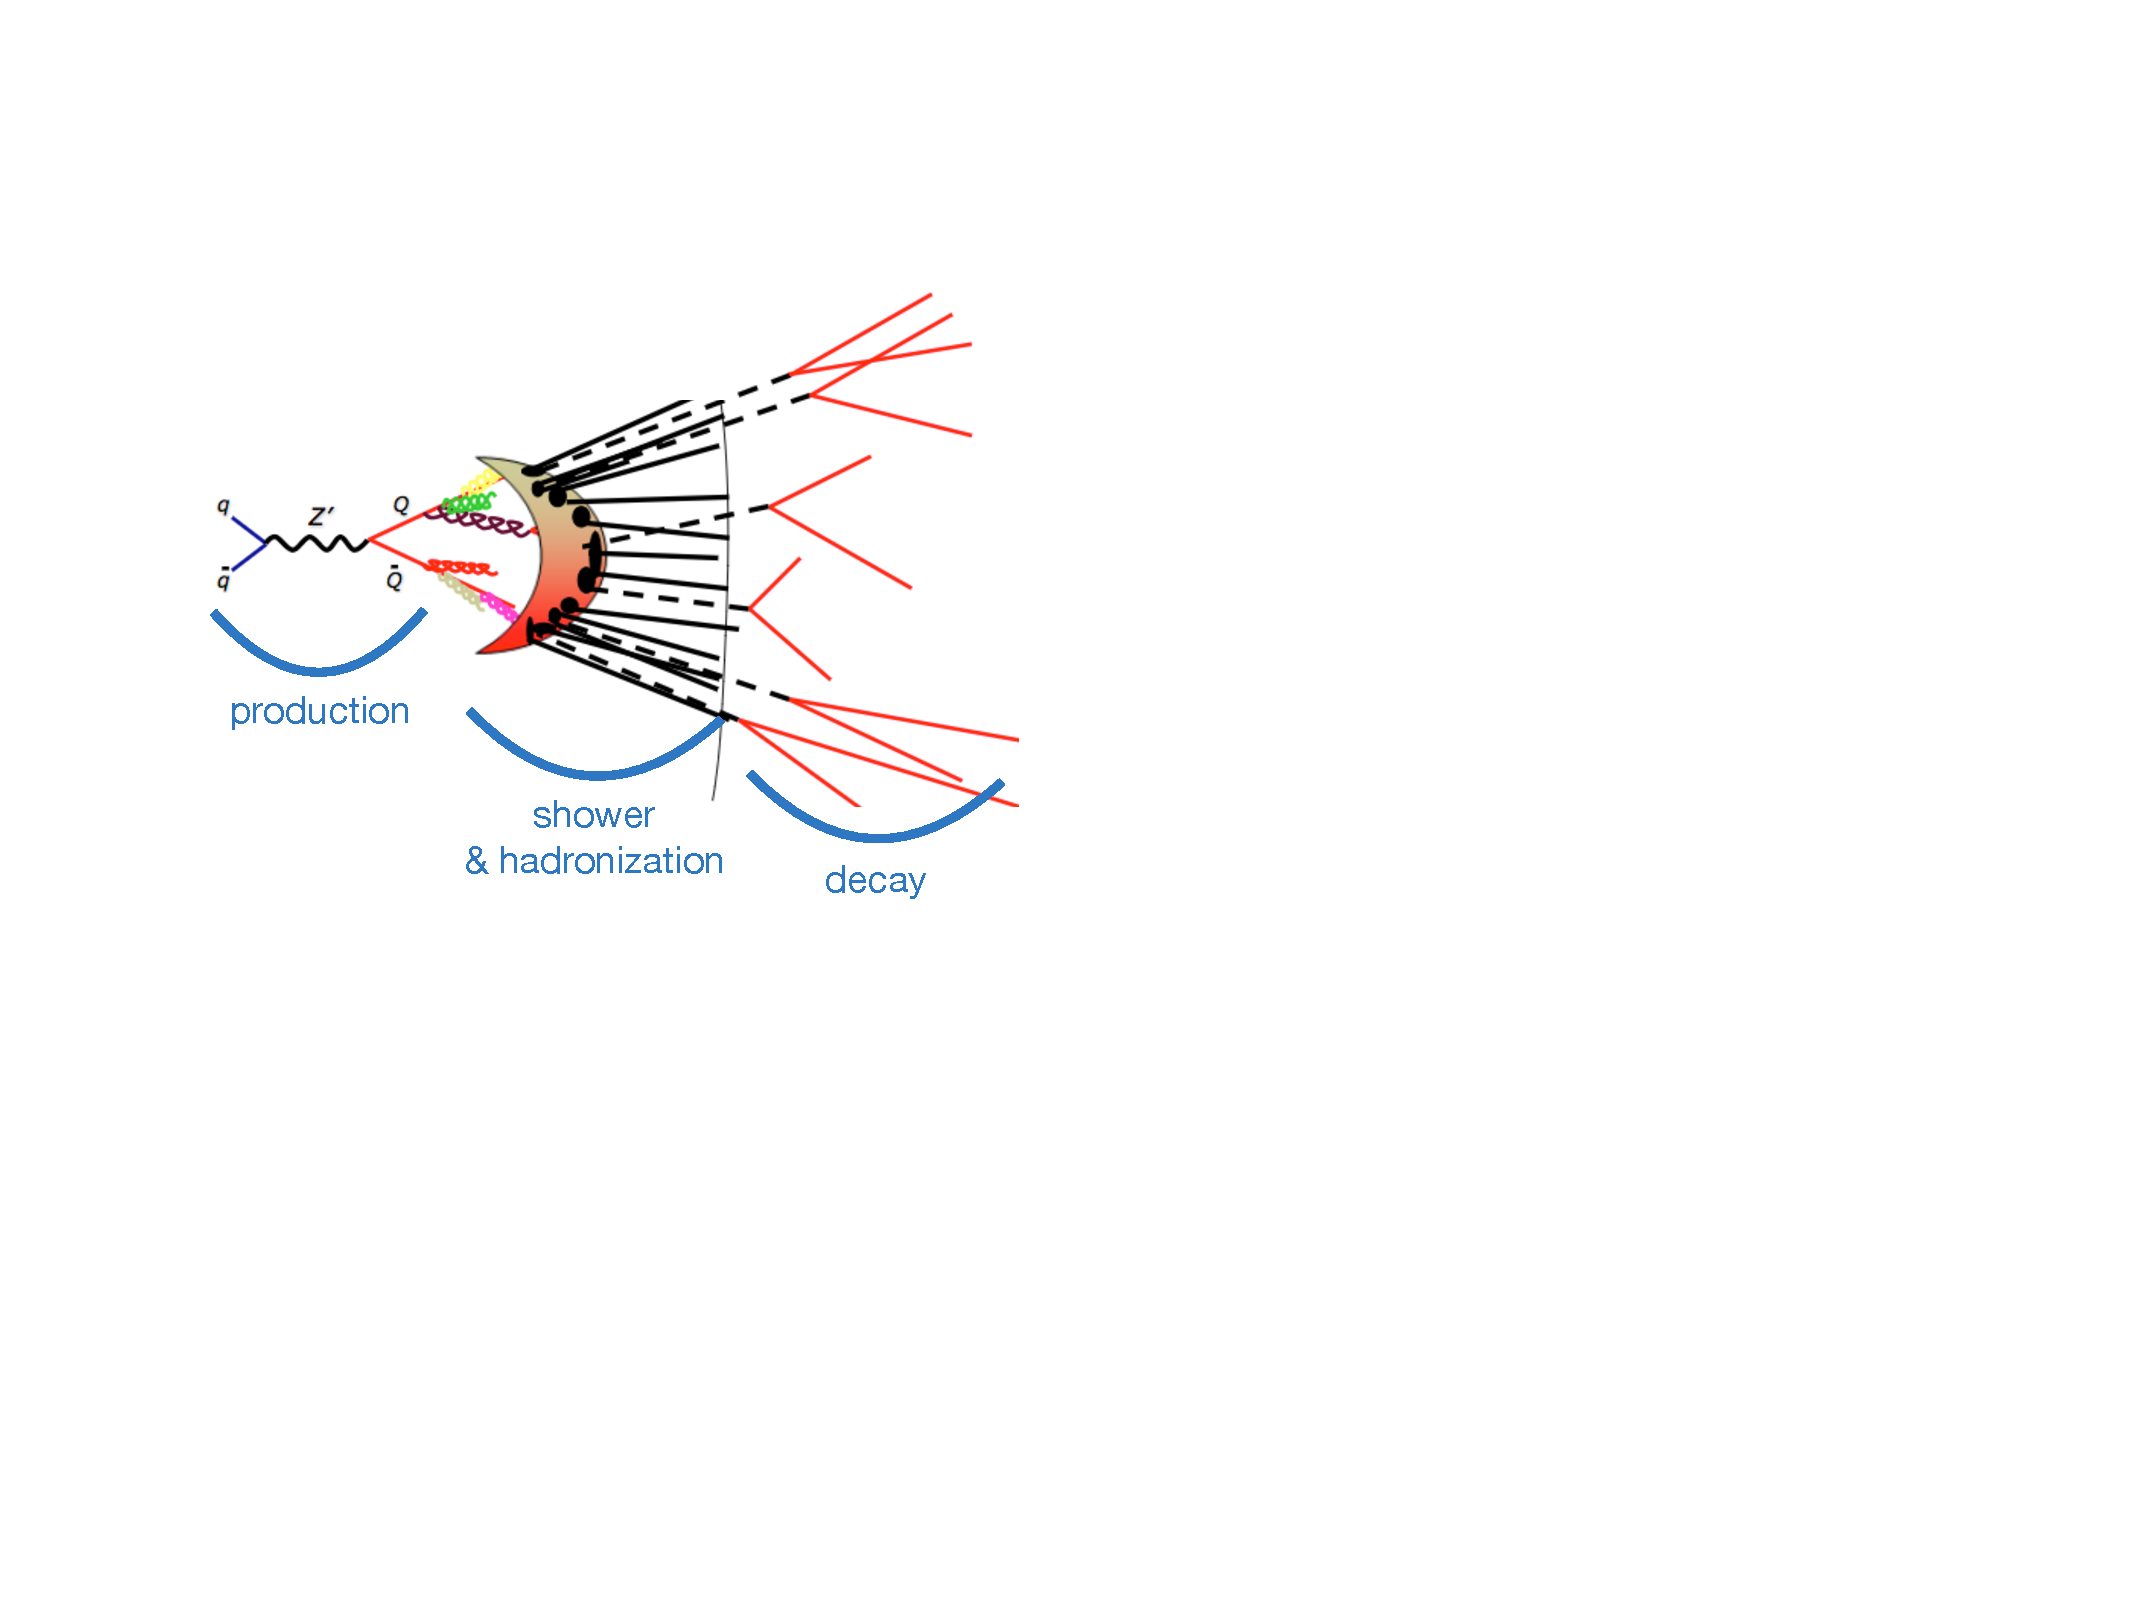
\includegraphics[width=0.6\textwidth]{figures/DS_diagram}
\caption{Schematic representation of a dark shower event, in this case from hidden valley model with a $Z'$ production portal. Figure adapted from \cite{Strassler:2008fv}.\label{fig:showerdiagram}}
\end{figure}
\end{enumerate}

A priori it is typically possible to construct a model by picking and choosing an ingredient from the menu of options for each of the three components outlined above. This is an enormous model space, and it may appear daunting to construct searches capable of capturing all possibilities. On the other hand, the signatures of these models are often so striking that they enable powerful, inclusive searches, sensitive to a very large portion of this overall model space, provided that triggers allow the event to be recorded. Toward this end it is useful to observe that dark shower events have the following generic features:
%
\begin {enumerate}

\item Events will have a variable and potentially large multiplicity
  of LLPs.  The number of produced particles of various dark species
  depends on the details of the parton shower and/or hadronization, as
  in QCD, and will vary from event to event.  Typically there will be
  more than two LLPs per event.

\item The BSM species produced in dark showers exhibit a hierarchy of
  proper lifetimes.  This could result in production of e.g. mostly
  prompt particles with a few displaced decays; mostly invisible
  detector-stable particles with a few displaced decays within the
  detector; or anything in between.

\item LLPs will not generically be isolated, i.e., will often appear
  within $\Delta R \lesssim 0.4$ of other LLPs and/or prompt objects
  (such as the decay products of short-lived species originating from
  the same shower).

\item The energy flow in the event will reflect the evolution of the
  BSM parton shower, and will thus look non-SM-like.  For instance,
  hidden sector jets may be either narrower or broader than QCD jets,
  depending on the hidden sector gauge group and gauge coupling.
  Additionally, SM particle multiplicity, i.e., the relative fractions
  of pions, kaons, etc. produced in a jet, will differ from QCD. 
While energy flow can be a powerful discriminant
to separate dark showers from the SM, at any stage from the trigger
level forward, it is model-dependent and must be assessed on a
case-by-case basis. Turning this around, it also implies that traditional (displaced) jet triggers do not suffice to cover the general model space, and alternative trigger strategies (e.g.~track or muon multiplicity) are needed as well.

\end {enumerate}

The existence of $\gtrsim 2$ LLPs per event, and indeed frequently
$N_{LLP}\gg 2$, generally ensures that these events can be easily
distinguished from background if they can recorded on tape and subsequently reconstructed.
However, the unique features of events with dark showers require new
strategies to ensure that this class of theories is actually captured
by the trigger.  In particular, non-isolation and the hierarchy of
proper lifetimes can result in qualitatively novel collider signatures
that require novel triggering ideas as well.  Meanwhile, event-level observables such as non-SM-like energy flow or particle multiplicity are potentially powerful but highly model-dependent discriminants, and must be considered on a case-by-case basis.
We discuss the strengths and shortcomings of existing triggers and off-line strategies in Secs.~\ref{sec:darkshowertrig} and \ref{sec:darkshowerreco}, as well as a number of new ideas. An executive summary of our main points and recommendations is provided in Sec.~\ref{sec:darkshowersummary}. The chapter concludes with a collection of example models for which 
Monte Carlo event samples currently are available (see Sec.~\ref{sec:darkshowermodels}).

\section{Production}
\label{sec:darkshowerprod}

Events with dark showers generically begin with the pair production of dark
partons $Q_D$.  In most cases the two produced partons will be of the
same species, but this does not necessarily need to be true.
For clarity and simplicity, we will confine ourselves to the
case where $Q_D$ is a SM singlet.
Then the production modes for $Q_D$ can be simply related to the
production modes discussed for neutral LLPs in the Simplified Model
chapter, \ref{sec:proposal}.  In particular, the most relevant production modes are:
%
\begin{itemize}

\item {\bf Heavy Parent (HP):} Pair-production of a SM-charged heavy
  parent $X_D$, which subsequently decays via $X_D\to
  Q_D+\mathrm{(SM)}$.  The SM quantum numbers of the parent $X_D$, together with its mass,
  control both the overall production cross-section and the typical prompt
  accompanying  objects in the event. Depending on the lifetime of $X_D$, showering can begin before or after its decay. 
  The model of \cite{Schwaller:2015gea} features this production
  mechanism, 
  where the parent $X_D$ is a heavy scalar carrying both color and
  dark color charges. After QCD pair-production, the mediators decay
  into a visible jet and a dark shower each.


\item {\bf Higgs (HIG):} Production in exotic Higgs decays, $h\to
  Q_D\bar Q_D$.  
%
 As the Higgs boson provides an especially sensitive window onto low-mass dark sectors, this production mechanism is one of the best-motivated at the LHC \cite{Strassler:2006ri,Curtin:2013fra}. In particular, Higgs portal production is the dominant production mechanism in many Twin Higgs and
  related models of neutral naturalness~\cite{Craig:2015pha,Craig:2016kue,Curtin:2015fna}.  The Higgs boson determines the overall mass scale of the event, often
  awkwardly low for LHC triggers, while the branching fraction remains a free parameter.  As discussed in Sec.~\ref{SM:secProduction_modes}, the SM Higgs has a characteristic set of accompanying prompt
  objects, which can extend trigger options.
%
As also emphasized in Sec.~\ref{SM:secProduction_modes}, this category also encompasses production through parent Higgs-portal scalars, which may be either heavier or lighter than the SM Higgs.

\item {\bf $Z'$ (ZP):} Here a new $Z'$ boson couples to both SM and hidden sector
  states, such that the production mode is $q\bar q \to Z'\to
 Q_D\bar Q_D$. This scenario was developed in the original Hidden Valley models \cite{Strassler:2006im,Han:2007ae}, and considered again recently in \cite{Cohen:2015toa}.  The $Z'$ mass determines the overall mass scale, while production cross sections depend on its couplings to both SM and hidden sector states.  The only typical accompanying objects are ISR radiation.

\item {\bf Charged current (CC):} Here the parent dark states couple to the SM through the neutrino portal, $\mathcal{O}_{int}=HL \mathcal{O}_{\mathrm{dark}}$.  When the dark states carry charge under a dark gauge group, this coupling requires (at least) two dark states, one fermionic and one bosonic; for instance, if the dark sector contains both scalar and fermionic fundamentals, $\phi$ and $\psi$ respectively, then one can construct the dimension five interaction $\mathcal{O}_{int} = HL\phi^* \psi$.  This production mode has not been well studied in the literature.  It is worth noting that given this dark field content, it is generically possible to also construct Higgs portal couplings, $\mathcal{O}_H = |H| ^ 2 |\phi|^2, |H|^2\bar\psi\psi$, which can generally include lower dimensional operators.

\end{itemize}
As we have taken $Q_D$ to be SM singlets, the first process discussed in Sec.~\ref{sec:proposal}, direct pair production, is
typically negligible.  Of course, if BSM mediators connecting the dark sector to the SM, 
like the $X_D$ and $Z'$ in the examples discussed above, are heavy enough to be integrated out at LHC scales, then the resulting higher-dimension operators can mediate direct pair production of $Q_D$.
Single production of $Q_D$ is generally suppressed, and in many cases impossible, in particular when $Q_D$ transforms nontrivially under an unbroken gauge group. In Abelian theories, single production of a dark gauge boson is possible, e.g. through a loop of heavy bi-charged matter; this gauge boson can then go on to shower.  In perturbative cascades, a single BSM state $Q_D$ may certainly be produced, but whether $Q_D$ goes on to produce one or more `showers' is highly dependent on the detailed kinematics of the event. 

In contrast with the simplified models in section~\ref{sec:proposal}, after a parton
$Q_D$ is produced it undergoes extensive evolution in the hidden sector, so that
there is no one-to-one connection between the initial $Q_D$ and
relevant detector objects.  Thus an event that begins with 2 partons may result in a final state that contains two pencil-like jets, each containing more than one displaced object; a spherical distribution of displaced objects; or anything in between.  

The most important consequences of production modes for our purposes are twofold.  First and most importantly, the production mode informs the types of prompt accompanying objects in an event, as well as determining overall event rate and energy scale.  These accompanying objects can be useful levers to distinguish signals from SM background, beginning at the trigger level. Secondarily, production modes rely on a mediator that couples the dark sector to the SM, which may be a BSM particle like a bifundamental $X_D$ or a $Z'$, or a SM particle like the Higgs boson. In many models, this mediator-SM coupling also ultimately governs the decay of the dark sector states back into the SM. This is the case for the examples of Refs.~\cite{Schwaller:2015gea,Strassler:2006ri,Strassler:2006im,Han:2007ae,Cohen:2015toa,Renner:2018fhh,Craig:2015pha,Craig:2016kue,Curtin:2015fna}, and is certainly the minimal possibility. It is worth mentioning, however, that decays may be governed by a different interaction than production.  As a simple perturbative example, consider the hidden abelian Higgs model. This theory can realize dark showers in a variety of ways; consider for concreteness the perturbative cascade decay chain $h\to ss, s \to Z_D Z_D$, which can yield collimated pairs of dark photons when $m_s\ll m_h$. In this case a Higgs portal interaction governs production, but the long-lived $Z_D$ decays back to the SM through a separate vector portal interaction. 

\section{Shower}
\label{sec:darkshowershower}

\subsection{Motivation}

A familiar feature of QCD is the formation of jets, sprays of approximately collinear hadrons arising from a parton emitted in a hard scattering process. The physics of jet formation is independent of hadronization or confinement, originating in the singularities of the weakly coupled theory at short distances~\cite{Sterman:1977wj}, where the 't~Hooft coupling $\lambda \equiv g_s^2 N_c \ll 1$. The differential probability in perturbation theory for a quark to radiate a gluon carrying a small energy fraction $z$ at small angle $\theta$ is
\begin{equation}
\label{eq:scsplit}
  P(z, \theta)\, dz\, d\theta \sim \frac{\lambda}{4\pi^2} \frac{dz}{z} \frac{d\theta}{\theta},
\end{equation}
independent of the underlying hard process. The logarithmic divergences at $z, \theta \to 0$ indicate that perturbative theories favor radiation that is \emph{soft} (low energy) and \emph{collinear}. This enhanced emission of collinear radiation is the source of jets, even in theories that do not confine at all, such as the perturbative, conformal Banks--Zaks gauge theories~\cite{Banks:1981nn}. (See~\cite{Larkoski:2017fip} for a brief and clear recent introduction to jet physics emphasizing the role of scale invariance.) The large logarithms appearing in these calculations can be numerically resummed through Markov Chain algorithms, leading to the \emph{parton showers} widely used to model jets in Monte Carlo simulations. 

In the limit of strong 't~Hooft coupling\footnote{When making this and similar statements below, we always implicitly mean the coupling at the energy scales being probed by a given measurement. For example, while QCD does become strongly coupled near its confinement scale, if one only ever talks about jet masses and energies at much larger scales, treating the theory as weakly coupled is justified.} ($\lambda \gg 1$) perturbation theory breaks down; soft and collinear radiation are no longer enhanced over more general radiation at wide angles. In QCD, the coupling gradually runs strong in the infrared, but other gauge theories (which could  be realized in nature as hidden valleys~\cite{Strassler:2006im}) with an intrinsically large 't Hooft coupling persisting over a wide energy range exist. Such theories can be understood with the use of gauge/gravity duality. Examples may be conformal, e.g., strongly coupled $\mathcal{N} = 4$ super-Yang--Mills, or confining, e.g.,~\cite{Polchinski:2000uf, Klebanov:2000hb}. Such large-$\lambda$ theories were conjectured to lead to spherical event shapes~\cite{Strassler:2008bv}, a result that has been directly proven for strongly-coupled large-$N_c$ CFTs~\cite{Hofman:2008ar}. At colliders, these spherical events would lead to characteristic soft unclustered energy patterns (SUEPs)~\cite{Kang:2008ea, Harnik:2008ax, Knapen:2016hky}. An illustration of the range of event shapes from jets to SUEPs is shown in Fig.~\ref{fig:eventshapes}.

\begin{figure}[t]\centering
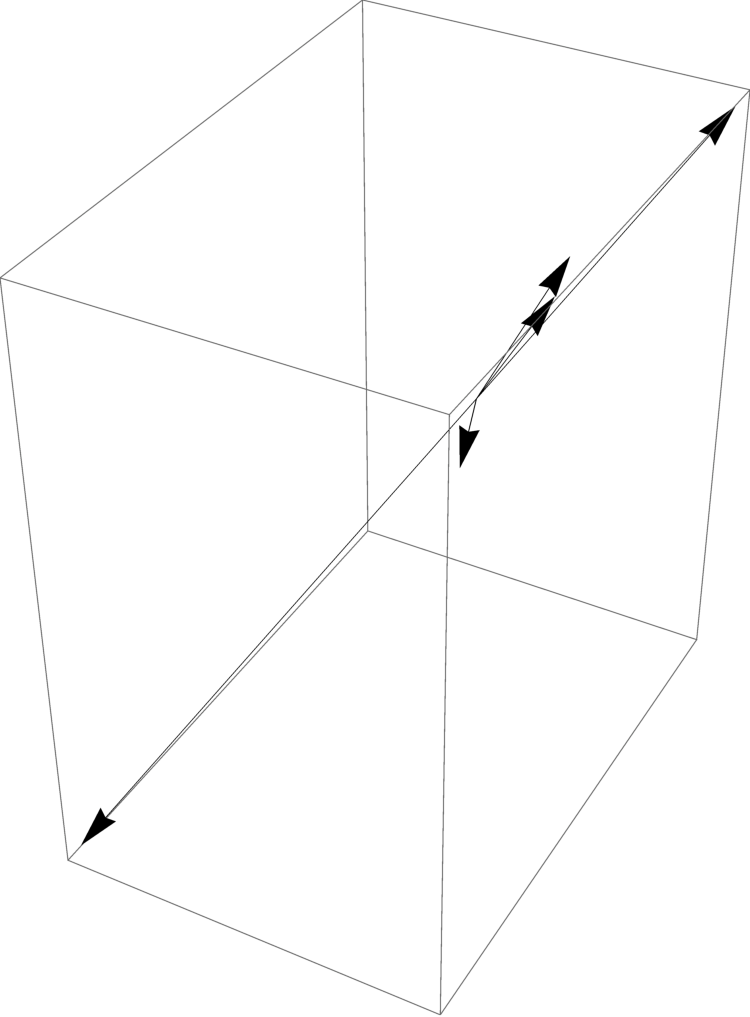
\includegraphics[width=0.25\textwidth]{figures/DS_KKexample_event1.pdf}
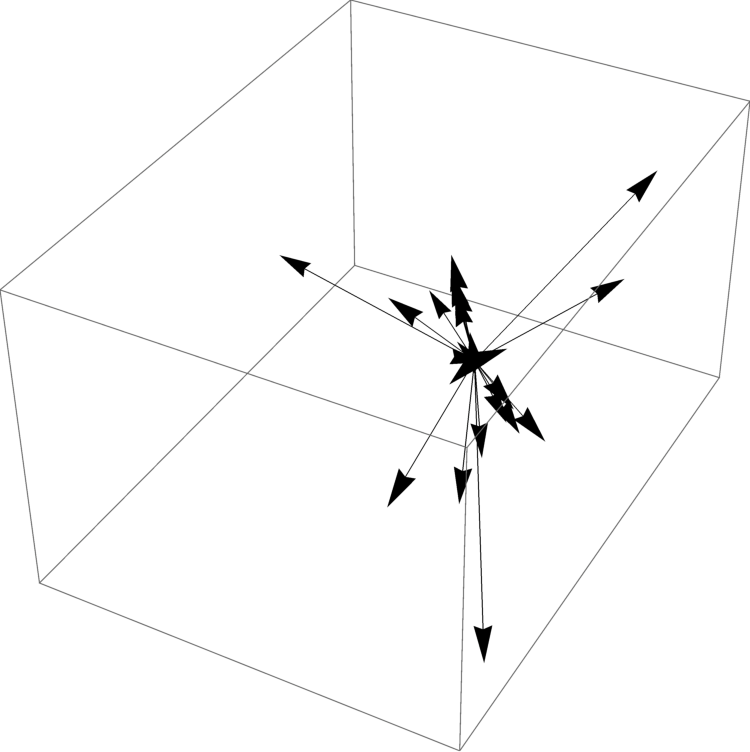
\includegraphics[width=0.31\textwidth]{figures/DS_KKexample_event2.pdf}
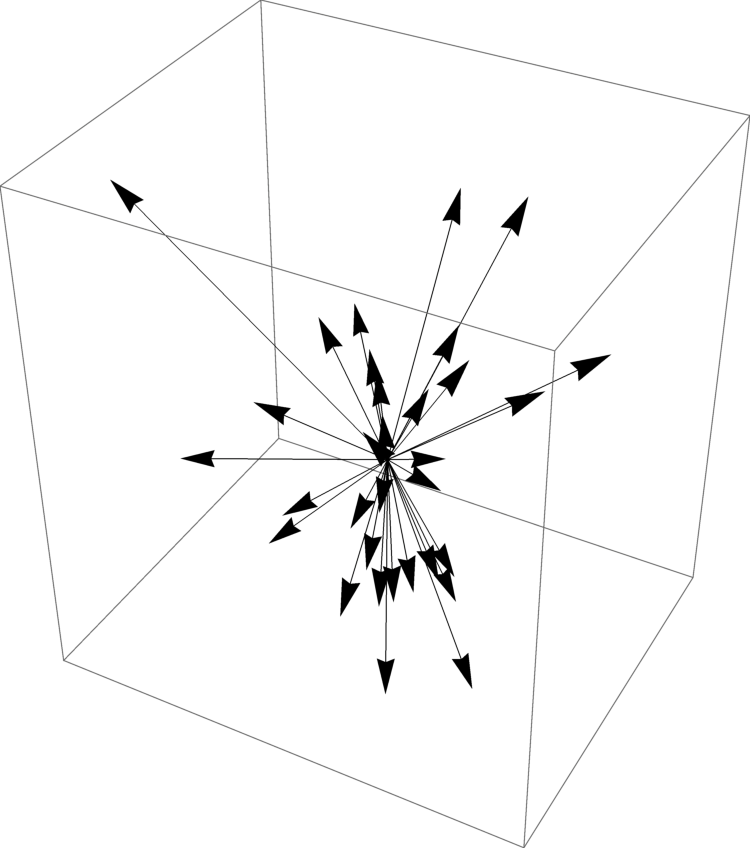
\includegraphics[width=0.31\textwidth]{figures/DS_KKexample_event3.pdf}
\caption{Illustrations of event shapes, from jetty (left) to spherical (right) with an intermediate event in the middle. The values of Sphericity and Thrust are:~(left) Sphericity = 0.00636, Thrust = 0.991; (center) Sphericity = 0.530, Thrust = 0.706; (right)  Sphericity = 0.940, Thrust = 0.521. \label{fig:eventshapes}}
\end{figure}


Thus we have two well-understood regimes, jets at $\lambda \ll 1$ and SUEPs at $\lambda \gg 1$. There is a gap in the middle, when $\lambda \sim 1$ over a wide range of energies. Both perturbative QCD and gravitational duals approach strong coupling in this regime (from different sides) and cannot be trusted to give accurate predictions, for some questions perhaps not even qualitatively so.

This regime is of interest because we want to ensure that LHC experiments do not miss a hidden valley signal simply because it looks different than expected. We should aim to be able to trigger on and analyze these events. While sufficiently long lifetimes may provide useful trigger handles, theories at intermediate 't~Hooft coupling could also occur with prompt decays while still failing to provide the types of trigger handles typically associated with prompt hard production and decay. Given our inability to reliably calculate the predictions of this scenario, in this section we will take a pragmatic approach. We will push the two tools we have, perturbation theory and gauge/gravity duality, into a regime where we do not fully trust them. To the extent that their predictions overlap, one could gain confidence in the qualitative picture we obtain. Where they differ, one would hope that experimental strategies broad enough to encompass the range of possibilities would also be sensitive to poorly modeled scenarios. In the following we present some initial results, which we aim to improve and expand upon in future published work.


\subsection{Phenomenological models}

\subsubsection{Parton showers and their limits}

One can  approach the intermediate regime from the direction of weak 't~Hooft coupling using parton shower methods. The coupling is then a direct parameter of the model whose value is easy to vary. However, naively setting the coupling to large values will quickly lead to unphysical results. The reason is that the simplest derivation of parton shower evolution equations assume that the final state can be organized as a series of splittings where $z, \theta \ll 1$ at each iteration. Since the full matrix element for a given final state has no uniquely-defined splitting history associated with it, this soft, collinear condition needs to hold as a function of the final state kinematics alone. As the coupling is increased, the increased showering probability means that the chance of populating the phase space while violating these conditions increases. Regions of phase space without nominal soft-collinear enhancements (but in truth  populated with comparable probability) will end up underpopulated, leading to more jetty events than the underlying theory actually predicts.

\begin{figure}[tb!]
	\centering
	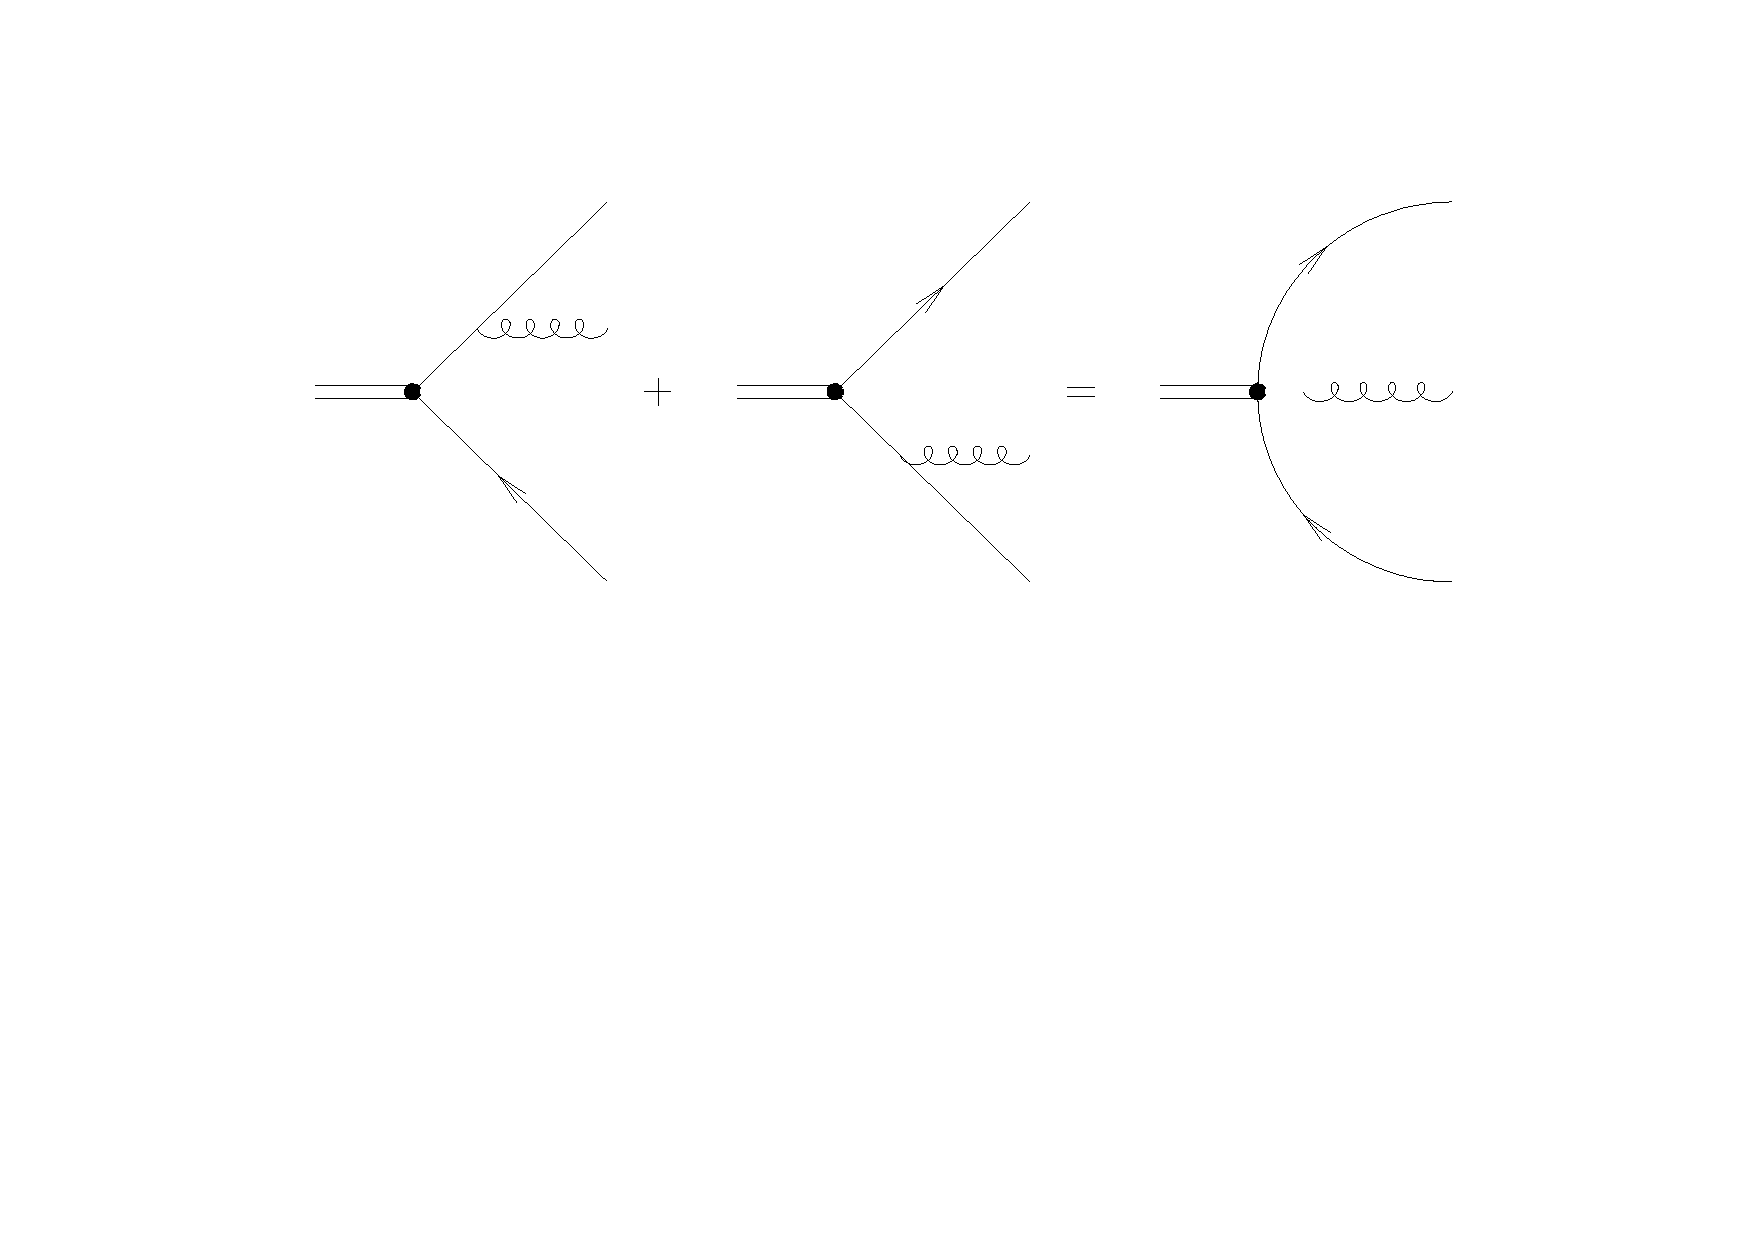
\includegraphics[width=0.48\textwidth,trim={5cm 11cm 5cm 3cm},clip]{figures/DS_dipole.pdf}
	\caption{Schematic view of a $2 \to 3$ branching process, with the initial 2-particle state approximated as a localized dipole. (Figure courtesy of \cite{Ellis:1991qj}.)}
	\label{fig:dipoleant}
\end{figure}

Things can be somewhat improved by a more careful consideration of parton shower methods. It is currently known how to implement iterated corrections allowing one to relax one, \emph{but not both}, of the inequalities given above. Implementations which allow for the correct inclusion of finite-$z$ (but small-$\theta$) effects can be accomplished by extending the approximation of Eq.~\eqref{eq:scsplit} with terms non-singular in $z$.

If we have reason to believe that the wide-angle structure of dark showers will be more critical to detecting models in the transition region, sacrificing finite-$z$ corrections for a better understanding of the finite-$\theta$ region is preferable. This requires going beyond the $1 \to 2$ splitting picture of Eq.~\eqref{eq:scsplit} as information about multiple particles in the event must be encoded. A known solution is to phrase the shower in the language of $2 \to 3$ evolution kernels~\cite{Giele:2007di}, where radiation is treated as coming from dipoles rather than individual charges, as in Fig.~\ref{fig:dipoleant}. Necessarily more complicated, in this approach the splitting function describing  the emission of a gluon with momentum $p^\mu$ is then expressed as
\begin{eqnarray}
  P(p_r^\mu)\, d\Phi_r &\sim&
    \frac{\lambda}{s_{ij}}
    \left[\pqty{ 1 - \frac{s_{ir}}{s_{ij}} - \frac{s_{rj}}{s_{ij}} }
          \pqty{ \frac{2s_{ij}^2}{s_{ir}s_{rj}} + \frac{s_{ir}}{s_{rj}} + \frac{s_{rj}}{s_{ir}} }\right.\\
          &&{} \left.  + \text{non-singular}\right]  d\Phi_r, \\
  \qcomma s_{ij} &=& (p_i + p_j)^2.
\end{eqnarray} 
for the process $a + b \to a + r + b$. Features related to the expected broadening of jets at larger coupling will be well-modeled deeper into the transition region with a dipole shower. Angular structure will be correctly reproduced even at larger couplings while final-state energy sharing of collinear particles becomes increasingly untrustworthy. When some sort of angular localization of energy flow can be expected (i.e., soft-collinear enhancements are still present) the corrections at finite splitting angle may still provide a good approximation.

\subsubsection{Gauge/gravity duality: spheres to jets}
\label{sec:darkshowerKK}

Gauge/gravity duality allows calculation in $\lambda \gg 1$ theories with spherical events, from which we extrapolate toward the $\lambda \sim 1$ regime. The simplest case is AdS/CFT duality, where events are perfectly spherical~\cite{Hofman:2008ar}. AdS space is a warped product of a $(3+1)$D Minkowski space with an infinite fifth dimension. To obtain a theory with a discrete spectrum, we cut off the fifth dimension of AdS space at a hard wall or \emph{IR brane} as in Randall--Sundrum (RS) models~\cite{RandallSundrum:1999}. Five-dimensional fields then decompose into a tower of 4D Kaluza--Klein (KK) modes (dual to hadrons in the gauge theory), each with an associated wave function in the fifth dimension. This wave function, as well as the 4D mass, is calculated by solving the equations of motion up to quadratic order. The couplings between 4D mass eigenstates are proportional to the overlap of their wave functions in the fifth dimension. 

Heavy KK modes decay to lighter modes, which decay to still lighter modes, populating a cascade of particles. The case of a flat (unwarped) extra dimension yields sinusoidal wave functions and modes with linearly spaced mass. In this case, the \emph{KK number} is a conserved discrete momentum in the fifth dimension, and KK modes decay only to daughters at threshold. The RS model breaks translation invariance in the fifth dimension, so KK number is no longer exactly conserved and a variety of decays are possible. Nonetheless, for the simple model of a bulk cubic coupling, KK number is still approximately conserved, as illustrated in Fig.~\ref{fig:BR}, left panel, and the sum of the two daughter modes is approximately equal to the KK mode of the parent. At each step of the cascade, daughter particles have small momentum. This results in spherical event shapes, with no highly boosted daughters~\cite{Csaki:2008dt}. Here we have studied a scalar field with a $\Phi^3$ interaction for simplicity, with the expectation that qualitative features of the event shapes persist in more realistic models.

To push our toy model into the jetty regime, we introduce interactions that explicitly break KK number themselves. We continue to study the simple case of a scalar field, but now to move toward jettier events, we include the $\Phi^3$ interaction as a boundary term, restricted to the IR brane. As shown in Fig.~\ref{fig:BR}, right panel, this opens up a much wider range of possible decays with greater phase space, which lead to more variety in the resulting event shapes. We emphasize that moving the $\Phi^3$ term to the boundary is a simple toy model for the purpose of this section that accomplishes the goal of altering event shapes. However, it is not expected to be a good approximation of the dual of an actual confining gauge theory with smaller $\lambda$.

\begin{figure}[tb!]
	\centering
	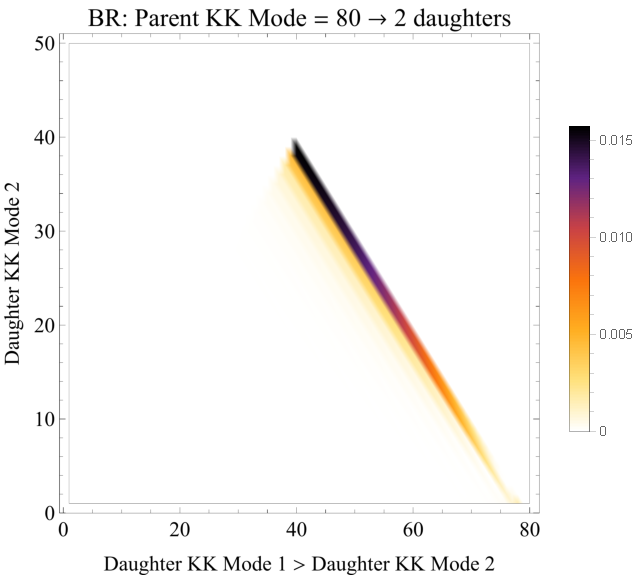
\includegraphics[width=0.48\textwidth]{figures/DS_KKBR_bulk.pdf}
	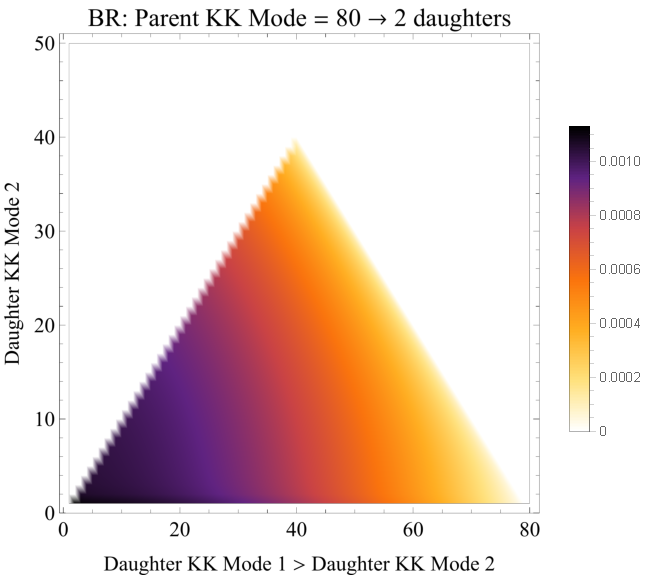
\includegraphics[width=0.48\textwidth]{figures/DS_KKBR_boundary.pdf}
	\caption{The branching ratio from a parent with KK-number 80 into two daughters for a cubic interaction on the bulk (left) or on the boundary (right). The nonzero probabilities occur along the line where KK-number is conserved for the bulk interaction, whereas the boundary interaction has non-zero probability to decay with large jumps in phase space. }
	\label{fig:BR}
\end{figure}

Although the IR brane interaction is used here as an ad hoc tool for generating less spherical events, we expect that similar results can be achieved in a more principled way. As $\lambda$ decreases toward $O(1)$ values, the expectation from gauge/gravity duality is that more bulk fields, dual to the many single-trace operators in the gauge theory, become light. This suggests that models with several interacting bulk fields are a more faithful toy model of the physics of the dual gauge theories at intermediate $\lambda$. Such models could be of interest for a wider set of questions than event shapes, as they move the AdS/QCD toolkit---always a toy model at best---somewhat qualitatively closer to QCD. Such models and their consequences will be studied in a forthcoming publication.

\subsection{Results}

We wish to characterize to what extent our available methods allow us to model the range of behaviors we might expect from new showering sectors. Since we do not expect collimated sprays of final state particles to be a sensible way of organizing information in the event in all cases, for our purposes here, we focus on observables that can be defined globally. In particular, we study a pair of event shape variables that have proven useful to both establish and provide precision data on the non-abelian nature of QCD.

Sphericity is defined as the scaled sum of the two smaller eigenvalues of the sphericity tensor
\begin{equation}
  S^{ab} = \frac{\sum_i p_i^a p_i^b}{\sum_i |\vec{p_i}|^2},
\end{equation}
where the sum is over all final-state particles in the event~\cite{Bjorken:1969wi}.  With the eigenvalues $\lambda_i$ defined in decreasing order,  we have $S = \frac{3}{2}(\lambda_2 + \lambda_3)$, which can take on the values $0 \le S \le 1$. Thrust is instead defined via a maximization procedure with respect to all possible axes in the event~\cite{Farhi:1977sg} ,
\begin{equation}
  T = \max_{|\vec{n}| = 1} \frac{\sum_i |\vec{n}\vdot\vec{p}_i|}{\sum_i |\vec{p}_i|}.
\end{equation}
Both observables essentially measure the divergence of an event from the pencil-like final-state structure of a $2 \to 2$ scattering process without making any direct reference to jets. 

Historically, thrust had the advantage of being infrared and collinear safe. In a given event, the change in the thrust from considering an additional radiated parton vanishes as the parton becomes soft or collinear to the thrust axis. Singular regions of phase space thus do not contribute to finite values of the thrust, and its measured distribution in QCD is well described by a perturbative calculation up to corrections that scale as $O(\Lambda_\text{QCD}/Q)^2$, where $Q$ is a high-energy scale associated with the total system being probed by the thrust. This is not the case for sphericity---specifically a perfectly collinear splitting will still change the value of the sphericity tensor. A perturbative calculation of the sphericity will then be divergent for finite values of sphericity, a divergence which can be tamed by either an explicit cutoff at the hadronization scale supplemented by a phenomenological hadronization model (the approach taken by Monte Carlo generators) or by absorbing it into a form factor (as done in analytic calculations). In either case $O(1)$ sensitivity is induced to the region of phase space dominated by non-perturbative hadronization effects. For our concerns, this difference can be turned into an advantage, as an observed difference between the two observables can act as a diagnostic of the sensitivity of our predictions to the non-perturbative parameters in the parton shower.

Events from models expected to provide a range of behaviors were generated. Extra-dimensional models with both bulk and boundary interactions were considered, with the former expected to yield very isotropic events. For the parton shower, a modified version of the VINCIA dipole-antenna parton shower~\cite{Fischer:2016vfv} is used, in which an $SU(N)$ gauge theory with only light quarks showers and hadronizes into light mesons with masses $m_{\pi_v}/\Lambda_v \sim m_\pi/\Lambda_\text{QCD}$. Coupling boundary conditions and one-loop running were then varied while adjusting shower cutoffs to ensure that couplings remain perturbative throughout the parton shower.

\begin{figure}[tb!]
	\centering
	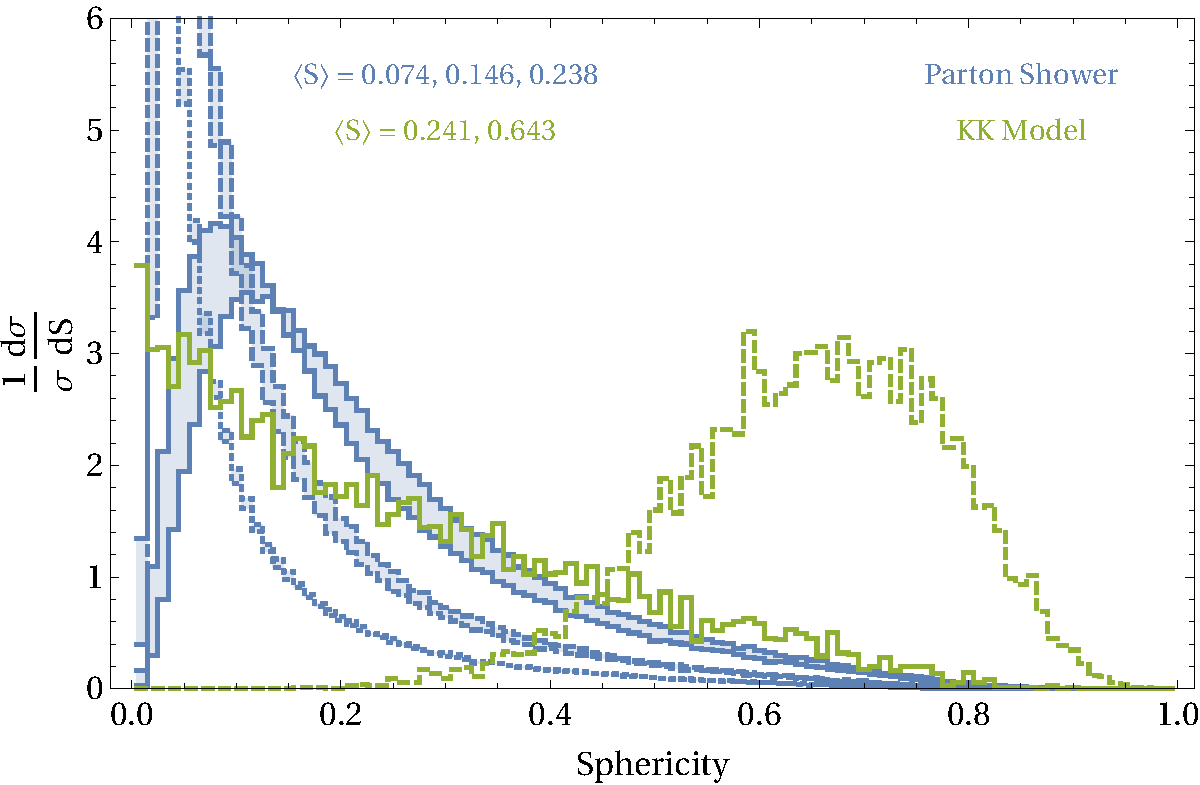
\includegraphics[width=0.48\textwidth]{figures/DS_comparison_sphericity.pdf}
	\hspace{5pt}
	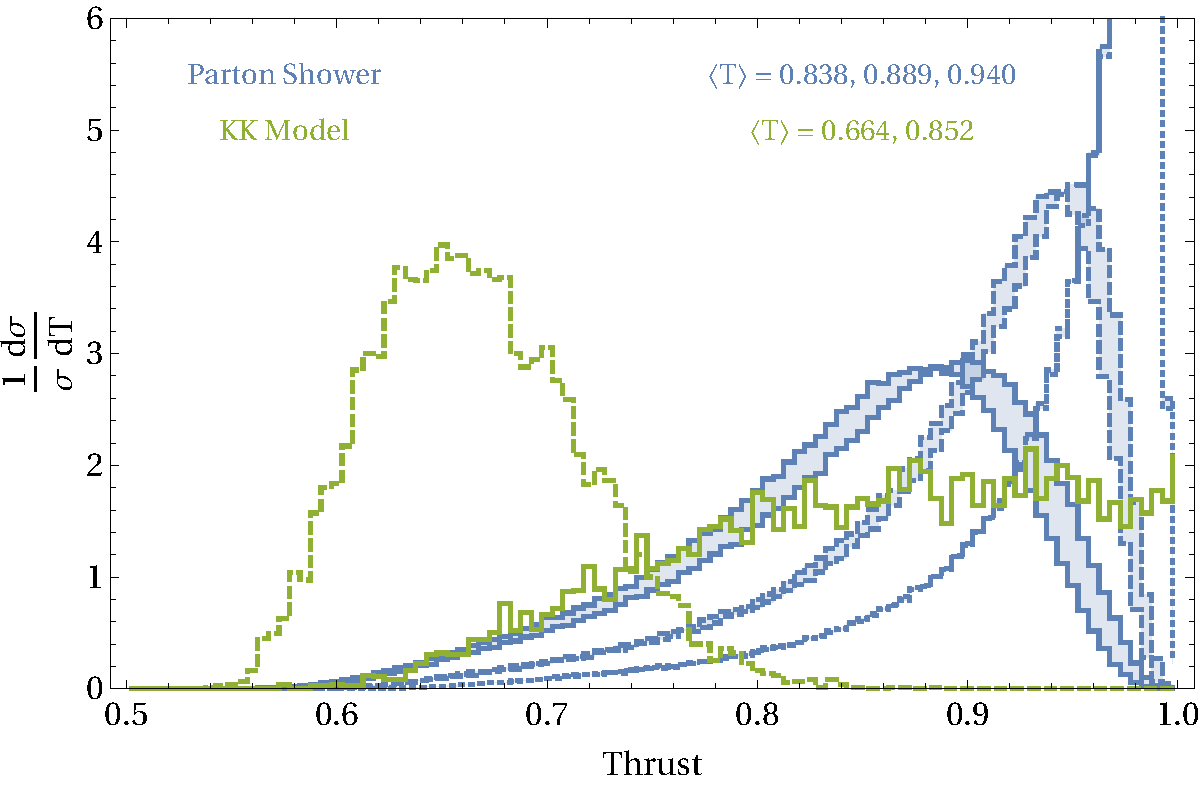
\includegraphics[width=0.48\textwidth]{figures/DS_comparison_thrust.pdf}
	\caption{Comparison between accessible ranges of parton shower and AdS/CFT-inspired models (labeled ``KK model'') for sphericity and thrust. In the parton shower, the curves correspond to events produced at $\sqrt{s} = 100\Lambda$, with confinement scale $\Lambda$. The $\beta$ functions of the theories are tuned such that $g^2(100\Lambda)/4\pi$ is $0.06, 0.12, 0.24$ for the 3 distributions. In the KK model case, the dashed curve corresponds to a bulk interaction while the solid curve corresponds to a boundary interaction. Expectation values for all distributions are computed.}
	\label{fig:compplots}
\end{figure}

The results are summarized in Fig.~\ref{fig:compplots}, with the uncertainty in the parton shower distributions coming from considering transverse momentum and dipole virtuality shower ordering. The similar behavior of the two distributions indicates that sensitivity to non-perturbative effects from hadronization are not large.  The lowest sphericity/highest thrust distribution is fairly close to that expected from QCD, but a wide range of non-QCD-like behaviors is observable. A significant fraction of the range in these observables is covered by both the extra-dimensional and the parton shower approaches, with similar results for the boundary interaction KK model and the parton shower models.

\begin{figure}[tb!]
	\centering
		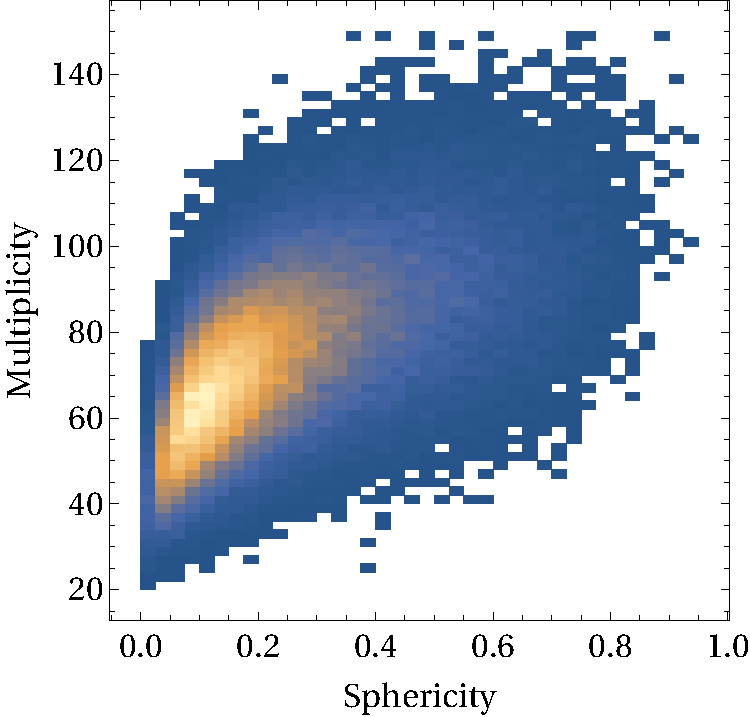
\includegraphics[width=0.35\textwidth]{figures/DS_sphericity_PartonShower.pdf}
	\hspace{5pt}
	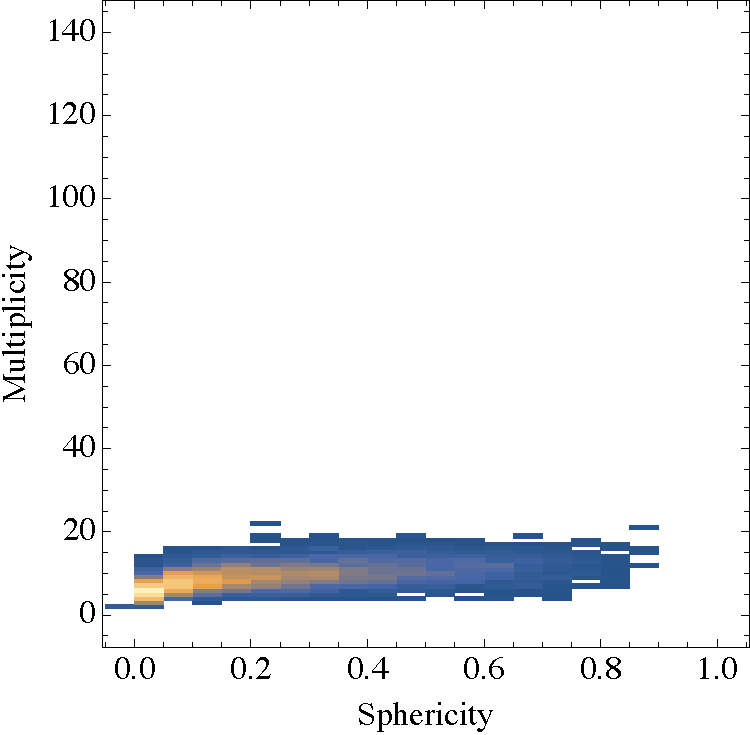
\includegraphics[width=0.35\textwidth]{figures/DS_sphericity_KK_bdry.pdf}
	\caption{Correlation between sphericity and hadron multiplicity for events generated with parton shower (left) and AdS/CFT-inspired models with boundary interaction (right).}
	\label{fig:compmult}
\end{figure}

Examining the behavior of observables that are perturbatively incalculable in the weakly coupled theory indicates that a degree of caution is warranted, however, with the two approaches giving qualitatively different results to certain questions. As an example, we look at the correlation between sphericity and total event multiplicity for the two closest parton shower and extra-dimensional models. Displayed in Fig.~\ref{fig:compmult}, we see that multiplicity is broadly correlated with sphericity in the parton shower, while being nearly sphericity independent for the KK model. Such qualitative difference seen between the parton shower and the extra-dimensional models warrants more detailed study of event behavior in the transition region, while both approaches would benefit from further consideration of how jet-level observables, whether physically well-justified or not, vary over their accessible ranges.

\section{Decay}
\label{sec:darkshowerdk}

In general, the mass spectrum of confining hidden sectors is poorly known, with the exception of a few special cases, like pure glue confining theories \cite{Morningstar:1999rf} and of course the Standard Model QCD sector. The dynamical process that is hadronization is even less understood, and one must typically resort to uncontrolled extrapolations from the measured fragmentation functions in the Standard Model. Moreover, even in well-understood examples,  states with different $CP$ and spin  quantum numbers will can have greatly different lifetimes \cite{Strassler:2006im,Juknevich:2009ji,Juknevich:2009gg}, a problem which can be further exacerbated if the hidden sector contains one or more approximate flavor symmetries. For concreteness we here primarily focus on the case where only one dark species has a detector-scale lifetime; other dark states may either  decay promptly to the SM or appear as MET.
A useful special case realizing this scenario is when all internal hidden sector decays are sufficiently rapid for nearly all hidden states to cascade promptly to the lightest state in the spectrum, which in turn decays to the SM. The discussion below is focused on the possible properties of this lightest hidden state which decays to the SM. We refer to it as ``the'' long-lived particle (LLP), keeping in mind that in complete models there may very well be multiple species of LLPs. It is therefore important to emphasize that \emph{experimental strategies should not be overly optimized} towards the naive assumption of a single LLP producing all visible decays, as it may not be generic. In particular, an inclusive experimental strategy should avoid making detailed assumptions about the distributions of proper lifetimes of long-lived states in the event.  


\subsection{Portals and branching ratios}
\label{sec:darkshowerportal}

The available decay channels and branching ratios of the LLP are critical both for the trigger strategy and the off-line analysis. In particular, for models where the LLP branching ratio to muons is not too small,  various (multi-)muon triggers can be very effective. At the same time, displaced hadronic decays tend to give more discriminating power in the off-line analysis, since they produce a larger number of tracks as compared to the leptonic modes. Since each event contains multiple LLPs, a single event can contain \emph{both} leptonic and hadronic vertices, where one uses the former for the trigger and the latter for off-line background rejection. For this reason it is not straightforward to interpolate  sensitivity between lepton-rich and hadron-rich hidden showers, since the optimal search strategy for the intermediate cases is qualitatively different from the strategies for the two extremes.

As a starting point for our exploration, we therefore recommend a small number of theoretically motivated decay portals, which cover the fully leptonic and fully hadronic cases, as well as two other intermediate scenarios. We focus our attention on operators of dimension four or five which do not induce additional flavor violation in the quark sector:

\begin{itemize}
\item Neutrino portal: If the LLP is a neutral, possibly composite, fermion $X$, it may decay through a small mixing with the standard model neutrinos. In this case, this state will predominantly decay through the $X\to \ell^+ W^{-(\ast)}$ and $X\to \nu Z^{(\ast)}$ channels and its decays will tend to be rich in leptons. The muon fraction in the final states depends on the mixing angle of the $X$ with the muon neutrino, which is model-dependent. However, even if this angle is accidentally small as compared to the mixing angles with electron and tau neutrinos, one still expects a muon in roughly $\sim10\%$ of all decays through the $W^{(\ast)}$ channel.
 
\item Hypercharge portal: It is plausible for a dark sector to contain a vector meson, whether it is an elementary $U(1)$ gauge boson or a composite (the analogue of the $\rho$ in the Standard Model). An elementary vector boson can be  copiously produced through decays of a hidden sector meson through a chiral anomaly, analogous to $\pi^0$ decay in the Standard Model.  Whether elementary or composite, such a vector state generically mixes with SM hypercharge through the kinetic mixing operator $\epsilon B^{\mu\nu}F'_{\mu\nu}$, where $F'_{\mu\nu}$ is the dark vector boson field strength.  The branching ratios of such a state then depend on its mass and can be extracted from data, as shown in table \ref{tab:branchingratios} (see e.g.~\cite{Meade:2009rb, Curtin:2014cca}). 

\item Higgs portal: In the same spirit, it is possible that a hidden sector scalar $S$ mixes with the Standard Model Higgs boson through the $S H^\dagger H$ operator. In this case, its SM branching ratios are proportional to $m_f^2$, with the caveat that non-perturbative effects modify the story substantially for $m_S\lesssim 5$ GeV. For $m_S\lesssim 1$ GeV, hadronic branching ratios can be obtained through chiral perturbation theory; however, in the intermediate range  $1\, \mathrm{GeV} \lesssim m_S \lesssim 5$ GeV, the theory uncertainties are substantial and we do not attempt to make any quantitative statements in this regime. (See \cite{Clarke:2013aya} and references therein.) As shown in table~\ref{tab:branchingratios}, the muon fraction predicted by Higgs portal decays is smaller than for the previous two portals, but it can still be relevant if the (non-isolated) muons from $B$-meson decays are taken into account. 

\item Gluon portal: The hidden scalar ($S$) or pseudo scalar ($a$) could also decay to the Standard Model through a coupling to gluons of the form $S \mathrm{Tr}G^{\mu\nu}G_{\mu\nu}$ or $a \mathrm{Tr}G^{\mu\nu}\tilde G_{\mu\nu}$. In this case the direct leptonic branching ratio is zero, although a small number of muons may still be produced in the hadronization process of the gluons. 

\item Photon portal: Similar to the gluon portal, the LLP could decay to two Standard Model photons through the $S F^{\mu\nu}F_{\mu\nu}$ or $a F^{\mu\nu}\tilde F_{\mu\nu}$ operators. The signature for this case is qualitatively different as from the previous four, since there no tracks at all, other than occasional photon conversions, and the signal is a trackless jet with high ECAL/HCAL ratio. 
\end{itemize}

If the lifetime of the LLP is $\lesssim \mathcal{O}(50)$ m, dark showers will generically give rise to multiple decays within the detector volume.  In table \ref{tab:branchingratiosevent} we show the probability for the Higgs and hypercharge portals to produce an event which contains at least 3 or 4 muons, as a function of the number of decaying LLPs in the event. Assuming the event has at least four LLP decays, a multi-muon trigger has good efficiency for the Higgs portal above the $b\bar b$ threshold\footnote{The importance of muons in decays which are rich in heavy flavor was emphasised in \cite{Strassler:2008fv}.} and for all masses for the hypercharge portal. (Again, this statement is LLP-lifetime dependent, and for sufficiently long-lived LLPs this strategy will break down as the probability of getting sufficiently large numbers of LLP decays within the detector becomes small.) This trigger strategy should also have good efficiency for  neutrino portal decays, although this scenario is more model-dependent. For the gluon and photon portals a different set of triggers is needed, as discussed below. The lesson is that multi-muon triggers do not suffice to cover all possible options, but could provide a reasonably generic trigger path for an important subset of the relevant models.

\begin{table}[h]\centering
\begin{tabular}{|c|cc|}\hline 
mass (GeV)  &photon &Higgs  \\\hline
0.5&0/0.4&0/0.09\\
1.2&0/0.35&/\\
8&0.08/0.16&0.25/0.02\\
15&0.1/0.15&0.3/0.05\\\hline
\end{tabular}
\caption{Probability of finding exactly one muon / two muons in one LLP decay through the photon and Higgs portals. For the lowest mass points, the branching ratios for the photon and Higgs portals were taken from \cite{Meade:2009rb} and \cite{Fradette:2017sdd} respectively. For the 8 and 15 GeV benchmark the hadronization was performed with Pythia 8 \cite{Sjostrand:2006za,Sjostrand:2007gs}.\label{tab:branchingratios}}
\end{table}


\begin{table}[h]\centering
\begin{tabular}{|c|c|ccccc|}\hline 
%&\multicolumn{5}{c|}{number of vertices}\\\hline
& mass (GeV) &3 decays&4 decays&5 decays&6 decays&7 decays  \\\hline
\multirow{ 4}{*}{\rotatebox{90}{photon}}&0.5& 0.36/0.36  & 0.53/0.53 &0.67/0.67&0.77/0.77&0.85/0.85 \\
&1.2& 0.29/0.29  & 0.44/0.44 &0.57/0.57 &0.68/0.68 &0.77/0.77\\
&8&  0.13/0.07 &0.23/0.13  &0.33/0.21&0.42/0.28&0.5	/0.35 \\
&15& 0.14/0.07  & 0.23/0.13 &0.33/0.2&0.42/0.27&0.51/0.35 \\\hline
\multirow{ 3}{*}{\rotatebox{90}{Higgs}}&0.5&  0.02/0.02&0.04/0.04 &0.07/0.07 &0.1/0.1 &0.13/0.13 \\
&8&  0.04/0.0 &0.09/0.02 & 0.15/0.04&0.23/0.07 &0.31/0.12 \\
&15& 0.11/0.02 &0.21/0.07 &0.33/0.13 &0.44/0.21 &0.55/0.31 \\\hline
\end{tabular}
\caption{Probability of finding at least 3 muons / at least 4 muons in an event for the photon and Higgs portals, as a function of the number of LLP decays. 
 Branching ratios and hadronization were determined as in Table~\ref{tab:branchingratios}.
\label{tab:branchingratiosevent}}
\end{table}

\subsection{Lifetime}
\label{sec:darkshowerctau}

Without additional model assumptions, the theory prior on the lifetime of the LLP is rather weak. We can however extract some insight from the generic scaling of the width of these particles as a function of their mass ($m$): for the Higgs and hypercharge portals $\Gamma\sim m$, for the ALP portals $\Gamma\sim m^3/f^2$ with $f$ the ALP decay constant, and for the neutrino portal $\Gamma \sim m^5/m_W^4$. The obvious trend is the lifetime rises as the mass decreases, steeply so for the case of the neutrino portal. It is furthermore important to keep in mind that the scalings above are lower bounds, and in many models the leading decay portal involves a higher-dimensional operator, leading to a stronger scaling. This is especially relevant in confining  models where the hidden states are composite particles. For example, in a pure glue hidden valley coupled though the Higgs portal \cite{Juknevich:2009gg}, the lightest glueball decays through the Higgs portal, but as it is created by the dimension-four combination of dark gluon field strengths $G^a_{\mu\nu}G^{a \mu\nu}$, its width scales as $\Gamma\sim m^7/\Lambda_{D}$, where $\Lambda_D$ is the scale of dark QCD. \SK{To fix, for Jessie}

An additional consideration is that the LLP can be discovered directly in (low energy) collider or beam dump experiments. Since the LLP has an irreducible production cross-section through the same coupling that governs its decay, collider experiments effectively impose a lower bound on the lifetime of these states. Beam and supernova constraints on the other hand rely on a displaced signal and constrain the lifetime from above. These bounds are however not typically applicable for masses above a few hundreds of MeV (for a summary of some of the latest constraints on the photon mixing and ALP portals see e.g. \cite{Ilten:2018crw} and \cite{Bauer:2017ris}).   However, particles that can be produced in sizable numbers at the LHC will in general be strongly enough coupled to the SM to face upper limits on their lifetimes from Big Bang Nucleosynthesis (BBN).   In most cases, this upper bound is essentially mass independent and requires $\tau\lesssim 1$ second, but this upper bound can be much weaker for lighter particles and/or particles that decay to hadron-poor final states.  For the ALP and hypercharge portals, prompt decays are currently allowed for masses all the way down to the electron threshold, though in the photon mixing case LHCb is expected to completely close this window below $\sim$ 100 MeV \cite{Ilten:2015hya,Ilten:2016tkc}. For the Higgs mixing portal scenario, current LHCb results from $b$ to $s$ transitions \cite{Aaij:2015tna,Aaij:2016qsm} already require $c\tau \gtrsim 0.5$ mm for masses below 4 GeV. For the neutrino mixing portal, lifetimes $c\tau\lesssim 10$ m are excluded if the mass is below 1 GeV and the mixing is predominantly with the electron and muon neutrino \cite{Deppisch:2015qwa}.

As argued above, if the mass of the LLP is larger than a few hundred MeV, their lifetime is only constrained from above by BBN. In the context of a dark shower topology, there is however a much more stringent upper bound to consider. In particular, to observe at least a handful of decays in the detector volume, the lifetime in the lab frame should satisfy
\begin{equation}
c\tau_{\text{lab}} \lesssim 10 \,\text{m}\times \frac{N_{\text{LLP}}}{N_{\text{decays}}}
\end{equation}
with $N_{\text{LLP}}$ the typical LLP multiplicity and $N_{\text{decays}}$ the number of observed decays in the detector. (The alternative case is obviously interesting as well, but maps onto the topologies with one or two displaced vertices, discussed elsewhere in this white paper.) For instance, for $N_{\text{decays}}\sim$ few and $N_{\text{LLP}}\sim \mathcal{O}(10)$ this implies $c\tau_{\text{lab}}\lesssim 50$ m. 

Near this heuristic upper limit in lifetime, the shower effectively gets stretched out over the detector elements, and it is useful to study how the decays are distributed over the different detector elements. We can use a toy monte carlo to make some simple estimates of this effect, by make the following simplifying assumptions: (1) the number of LLPs is Poisson distributed, (2) their decay length follows the usual exponential distribution with uniform average lifetime in the lab frame $c\tau_{\text{lab}}$ and (3) the angular distribution of the vertices is approximately spherical in the lab frame. Fig.~\ref{fig:detectorelements} shows the distribution of the number of decays occurring the tracker, calorimeter and muon chamber for two benchmark points. We hereby assume the approximate CMS geometry with the ``tracker'', ``calorimeter'' and ``muon chambers'' defined by $r<100\, \text{cm}$, $100\, \text{cm}<r<200\, \text{cm}$  and  $400\, \text{cm}<r<700\, \text{cm}$ respectively. We find that the number of decays in all detector components is roughly equal, with slightly more decays in the muon chamber for a higher number of LLP decays in the shower. The latter is easily understood from the larger size of the muon system as compared to the tracker and the calorimeter.  The qualitative point here is that tracker-based searches for multiple displaced vertices are likely to have reasonable sensitivity over the whole relevant lifetime range. For the longer lifetimes the sensitivity will necessarily degrade, although some of it can be recovered by adding the muon chamber to the analysis. Searches relying exclusively on the muon chamber or the calorimeter on the other hand will be less sensitive to a wide range of lifetimes. To quantify this effect more accurately, detailed simulations for specific benchmark models accounting for more realistic boost and $\eta$ distributions are certainly needed, although the relative importance of the tracker is likely to continue to hold. The displaced SUEP scenario is an interesting exception, as discussed in Sec.~\ref{sec:darkshoweremergingjets}. 

\begin{figure}
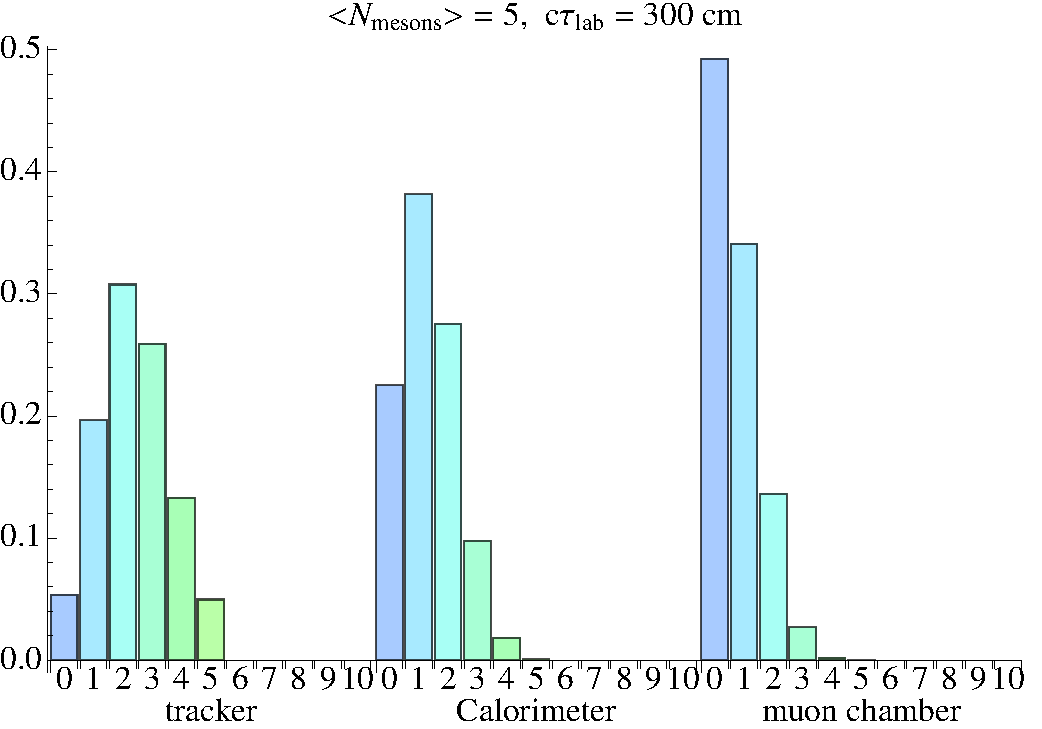
\includegraphics[width=0.45\textwidth]{figures/emerging_histograms_5.pdf}\hfill
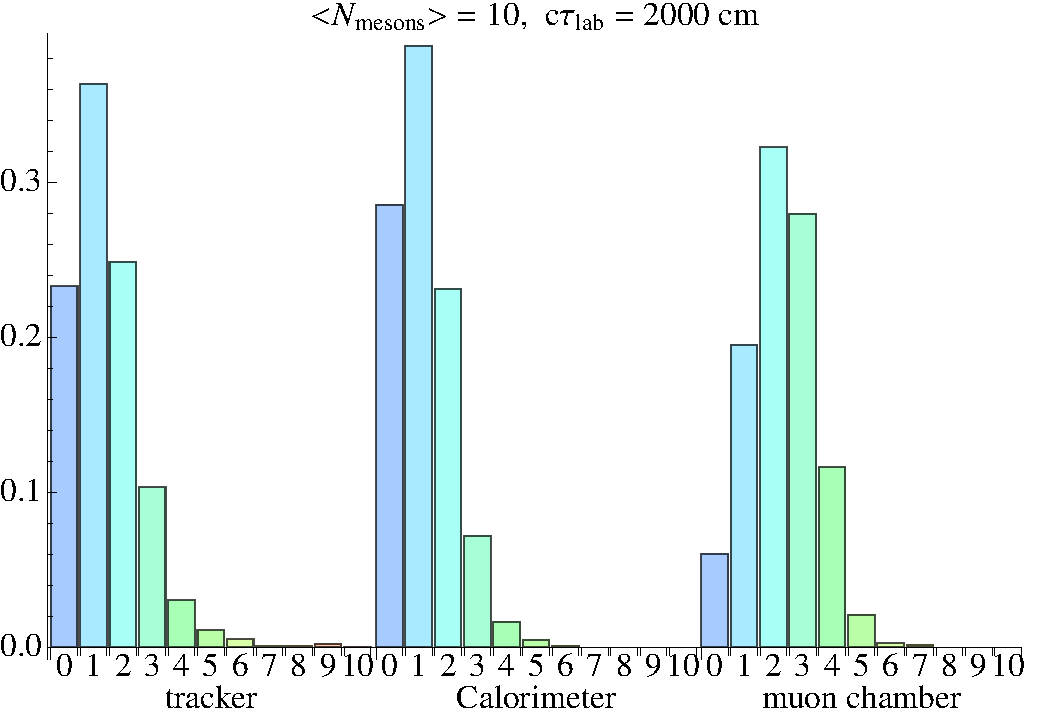
\includegraphics[width=0.45\textwidth]{figures/emerging_histograms_10.pdf}
\caption{Distribution of decays occurring in the various detector elements, for those events with more than three decays occurring in the fiducial volume.\label{fig:detectorelements}}
\end{figure}

\section{Trigger strategies}
\label{sec:darkshowertrig}

\subsection{General considerations}

Due to the immense diversity of hidden sector models, there is no trigger strategy which can comprehensively cover all options, nor is it straightforward to compile a list of such strategies. This problem is further compounded by the lack of available Monte Carlo simulations, except in a handful of special cases. 
Many of the considerations informing the trigger strategies discussed for singly and doubly produced LLPs in Secs.~\ref{tex/ExperimentCoverage} and \ref{sec:triggers}  apply to dark shower events as well.  However, the four characteristic features of dark showers laid out in Sec.~\ref{sec:darkshowerintro} can pose both additional opportunities and challenges:
\begin{enumerate}
\item \emph{The particle multiplicity can be high to very high.} This can in itself provide a very powerful trigger strategy, especially when the muon fraction in final states is appreciable, as discussed in Chapters \ref{sec:darkshowerportal}. For models where this is not the case or where the muons are too soft to fire the trigger, triggers relying on a large multiplicity of tracks or an overdensity of pixel hits could provide an alternative strategy. We will return to this discussion later in this section.

\item \emph{The hidden sector may contain states with wildly different lifetimes.} While this makes it  challenging to get a comprehensive grasp on the full space of possible event topologies, this feature provides interesting opportunities from the point of view of the trigger. For instance, often the most striking off-line signature is a set of displaced vertices in the tracker, which are notoriously challenging targets for the trigger. It is completely plausible that these vertices would originate from the decay of one species of hidden sector particles, while a second species decays either promptly or very displaced. This means that the event may very well come with prompt leptons, $H_T$ and/or an appreciable amount of MET or activity in the muon chamber.

\item \emph{The decay products may not be isolated.} Combining the two features above, we should prepare for the possibility that the objects we aim to use as trigger handles may not be isolated.  Especially for triggers on muons and (displaced) tracks, it is advisable to relax  isolation criteria as much as possible and instead rely on the presence of one or more additional objects to reduce rates as necessary. For example, one would expect that a trigger on two isolated muons would be less effective than a trigger on three or four non-isolated muons or a trigger with two non-isolated muons and a moderate amount of MET.  Non-isolation is likely to be a limiting factor for the acceptance of dark shower events in specialized triggers designed for singly- or doubly-produced LLPs. 

\item \emph{The energy flow in the dark shower may be non-standard.} This implies that a dark shower may be broader or narrower than SM QCD jets, and the momentum distribution of the particles in the shower may also differ substantially from QCD predictions. This means that triggers for (trackless) jets could be effective for some models, but would by no means capture the full range of possibilities. Since such $p_T$ distributions are very model-dependent, it is moreover sensible to keep object $p_T$ thresholds as low as possible, and instead rely on the high multiplicity by requiring multiple low $p_T$ objects, rather than a few high $p_T$ objects. 
\end{enumerate}

In summary, while some dark shower models will be very challenging to trigger on, this is not true for this class of models as a whole. While this is very far from universal, some models can readily be captured on the traditional MET, $H_T$ or lepton triggers. This means that these traditional triggers \emph{are an excellent place to start, but a bad place to stop.} Indeed, in the context of limited resources, it makes sense to first pursue the scenarios where the trigger is not a major challenge and use these scenarios to develop off-line reconstruction techniques. It is however crucial to follow up with more innovative trigger strategies. While this is largely still a topic of study, we can identify two categories of non-traditional triggers:
\begin{enumerate}
\item \emph{Triggers on displaced objects:} This type of trigger is notoriously challenging due to bandwidth and online computing limitations, but nevertheless a lot of progress has been made in the last few years. This is discussed in Chapters \ref{tex/ExperimentCoverage} and \ref{sec:triggers}.  For our purposes here, it suffices to note that (1) high multiplicity of LLPs in dark shower events can help provide excellent acceptance in such triggers, provided that (2) any isolation criteria in the trigger are not spoiled by shorter-lived objects in the event.

\item \emph{Specialized Triggers for dark showers:} There are a number of (speculative) ideas for triggers which exploit the high multiplicity and/or energy features of a dark shower, as described above, although this area is much less developed than the triggers on displaced objects. We will discuss these ideas for specialized triggers briefly in the remainder of this section, and comment on the unique capabilities of LHCb when it comes to triggering on dark showers. 


\end{enumerate}



\subsection{Specialized trigger ideas}

In this subsection we briefly highlight some proposals for specialized trigger strategies that inherently depend on the unique features of dark shower events.


\subsubsection{Multiplicity triggers}
\label{sec:darkshowertrigmultiplicity}

As emphasized  throughout this chapter, dark shower models can produce a high multiplicity of dark particles, ranging from several tens up to thousands of particles in the most extreme case. This motivates triggers that aim to minimize $p_T$ thresholds and instead exploit high particle multiplicity. The most obvious option is a suitable multi-muon trigger (three, four, or more muons), where the priority should be to avoid tight isolation criteria, if needed at the expense of increasing the muon multiplicity and/or $p_T$ thresholds. Prompt multi-muon triggers would, however, only capture (nearly) prompt decays, and it is critical to pursue the design and implementation of a trigger with good efficiency for displaced muons; see Sec.~\ref{sec:upgradesearch} for more on planned displaced muon triggers. 
%This would imply relaxing the condition that a matching track in the inner detector is found, again possibly at the expense of increasing the muon multiplicity and/or threshold, or by demanding a moderate amount of MET.   

Another way of exploiting the particle multiplicity is to trigger on an anomalously large number of tracks originating from the primary vertex. This would likely only work for prompt or nearly prompt decays, in models which produce a rather low muon fraction and/or a very soft $p_T$ spectrum. For this strategy to work, one must first pass the L1 trigger with MET, which can be provided by the shower itself or by initial state radiation (ISR). At the HLT it may be possible to count the number of tracks with the ATLAS FTK system or the future CMS hardware track triggers. Alternatively, if the tracks are too soft and the multiplicity high enough, it is possible to pass the HLT  by looking for an overdensity of hits in the inner most tracking layer, centered around the $z$-coordinate of the primary vertex \cite{Knapen:2016hky}.

\subsubsection{Substructure triggers}  
CMS already uses jet trimming at HLT level (see e.g.~\cite{Sirunyan:2017wto,Sirunyan:2017acf}), and we are aware of an effort within ATLAS to investigate the inclusion of substructure routines at the HLT level.   This may open up the possibility of using substructure techniques to distinguish between QCD jets and other types of showers already at the trigger level. This strategy could be helpful in cases such as photon-jets (dark showers that decay into SM photons), which can otherwise pose significant trigger challenges: substructure variables such as $n$-subjettiness \cite{Thaler:2010tr} and energy-energy correlations can be very effective at separating QCD jets, photons and photon-jets \cite{Ellis:2012sd,Ellis:2012zp}. In practical terms, this means that one may be able to use the relatively low threshhold jet/tau trigger for L1 trigger.  This could be followed by a HLT trigger that uses for instance the ratio of the energy deposited in ECAL over the energy in the HCAL or substructure variables.



It is worth noting that  substructure methods are fairly robust with respect to the lifetime of the dark shower final states, provided the lifetime is not too long compared to the size of the relevant detector subsystem. As long as the showering process itself happens quickly (dark showers often come from strongly coupled sectors), the separation between energy depositions in the calorimeter is already set and it does not matter if the decay products of the dark pion states are collimated themselves. In other words, as long as the dark pions are well separated, it does not matter that the dark pion decay products are nearly collinear. A clear difficulty with substructure triggers is that the actual dark showering process, and therefore the substructure, is theoretically only understood in a handful of example models, see Section~\ref{sec:darkshowershower}. While such a trigger is clearly valuable for a number of models, it is at the moment difficult to evaluate how broadly applicable it could be to different shower shapes.

\subsubsection{Non-isolated displaced vertex trigger in the ATLAS Muon Spectrometer}  
For sufficiently long-lived particles, fallback trigger strategies can be provided by existing ATLAS triggers that require a cluster of hits in the muon spectrometer (MS) \cite{Aad:2013txa,Aad:2013ela}.  As these triggers look directly for the presence of displaced objects and do not rely on any features of the rest of the event, they offer potential
sensitivity to signals dominantly produced at low mass scales.  The existing MS displaced vertex (DV) trigger requires at least three (barrel) or four (endcap) tracks in the MS \cite{Aad:2013ela}; a dedicated vertex-finding algorithm is run on these events at the analysis level.   Thus this trigger option offers good sensitivity to hadronic decays of particles with mass $\gtrsim 5 $ GeV, but cannot provide sensitivity to individual dileptonic or photophilic decays, nor to decays of LLPs with GeV-scale masses.

In Run I, LLP searches with displaced vertices in the MS relied on a trigger that recorded events where the displaced vertices additionally passed isolation requirements.  Specifically, events were required to have no tracks with $p_T>5 $ GeV in the inner detector within $\Delta R < 0.4$ of the displaced vertex, and the distance to the nearest jet (with $E_T > 30$ GeV) was required to be $\Delta R_j > 0.7$.  However, this isolation cut was not imposed for jets with anomalously large
energy deposition in the hadronic calorimeter, $\log_{10}(E_{\rm had}/E_{\rm EM}) > 0.5$ in order to improve acceptance for LLPs decaying in the outer edges of the hadronic calorimeter \cite{Aad:2013txa}.  This isolation requirement can limit acceptance for models with dark showers where multiple BSM species can spoil each other's isolation, especially in cases where the shower contains both short-lived as well as long-lived dark particles. It is an open question whether tracks from sufficiently displaced  vertices in the inner detector would contribute to the track veto, but particles that decay within the inner detector would be likely to spoil the isolation requirements through calorimeter deposits alone, unless their decays involved only muons.

New in Run II is a trigger on {\em non-isolated} clusters of hits in the MS \JS{experimental ref should go here but is not yet available, may be ready by white paper publication time}, which uses the same triggering algorithm for the muon system hits but does not impose isolation criteria.  The primary aim of this trigger is to enable background estimation for single DV searches \cite{Coccaro:2016lnz}, but it would also efficiently record dark shower signal events, regardless of event shape or event energy scale, provided at least one particle species in the shower has $m\gtrsim$ 5 GeV, decays to final states with at least 3 charged particles, and has reasonable probability to decay in the MS.  This trigger may be especially useful for high-multiplicity signals, where the probability for getting one particle to decay in the MS can become appreciable even for shorter-lived LLPs.  

\subsubsection{Capabilities at LHCb}

The LHCb detector is designed for studying displaced decays of SM mesons. This provides a good chance to look for dark shower events containing long-lived particles with lifetimes below the meter scale \cite{Strassler:2006qa}. Although LHCb does not yet have a dedicated trigger for dark shower events, many of the trigger strategies used for SM meson searches may be applied to dark shower signals. The LHCb detector is a single-arm forward spectrometer covering the pseudorapidity range $2<\eta<5$, which means the signals we are considering have typical $p_T$ that is much lower than the signals targeted by ATLAS/CMS. Hence, the LHCb signal trigger usually has much weaker $p_T$ requirements compared to an ATLAS or CMS search. This allows for better observation of dark shower events that come from the decay of light parent particles boosted in the forward direction, such as dark mesons from the decay of a light $Z'$.

For example, Ref.~\cite{Aaij:2014nma} searches for a pair of long-lived particles decaying into jet pairs. Although the signal is different from a dark shower, the trigger strategy in the search can be useful for dark shower events. The hardware trigger (L0) requires a single hadron, electron, muon, or photon with respective $p_T$ threshholds. For muons (hadrons), the threshholds are $p_T>1.48$ ($3.5$) GeV, and given the rapidity range of the signal, this corresponds to momenta $p> 6$ ($13$) GeV for muons (hadrons). These low $p_T$ requirements can thus keep soft and low-mass dark meson decays that can be hard to trigger at ATLAS/CMS. The software trigger contains algorithms that run a simplified version of track reconstruction and an identification of displaced tracks and vertices, and the first software stage (HLT1) requires a high quality displaced track satisfying the above $p_T$ requirement. In Ref.~\cite{Aaij:2014nma}, the final trigger stage (HLT2) further requires a displaced vertex with $\geq 4$ charged tracks, and either a $>2$ mm decay length in the transverse direction or the reconstructed vertex mass $>10$ GeV. Since the search focuses on $b$-quark final states, the HLT2 trigger also contains a multivariate algorithm to identify $b$-hadron decays. Although the trigger is designed for long-lived particles heavier than $10$ GeV scale, it is important to check if the same strategy is applied to even lighter particles or different decay final states.

For specific decay channels of dark mesons, we can also adapt triggers from  existing SM hadron searches that look for the same  final states \cite{Pierce:2017taw}. For example, if dark mesons decay into muon pairs or $c$-quarks, we can use similar triggers in the $K_s\to\mu^+\mu^-$ \cite{Aaij:2012rt} or $B^0\to D^+D^-$ \cite{Aaij:2016yip} searches to study the signal. A more recent muon trigger is used for the 13 TeV dark photon $A'\to\mu^+\mu^-$ search \cite{Aaij:2017rft}, where a muon with $p_T>1.8$ GeV is required at the hardware trigger level, and further quality cuts on the displaced vertex and muon identification are required. This search can be useful for dark mesons that decay through a kinetic mixing, in which muon final states have a sizable branching ratio.

Planned upgrades at LHCb are further discussed in Sec.~\ref{sec:LHCb_upgrade}.   These upgrades will make LHCb an even more powerful facility for studying LLPs, particularly in the low mass and short-lifetime regime, and further study of LHCb's capabilities for dark showers is well warranted.  

\subsubsection{Low pile-up data}

While Run 2 of the LHC has brought unprecedented opportunity for discovery with a large (expected > \mbox{120 $\text{fb}^{-1}$}) dataset of 13 TeV pp collisions, the ability to explore the energy frontier comes at a cost: high trigger thresholds and challenging experimental conditions may limit the sensitivity of LHC experiments to BSM models such as SUEP with soft and diffuse signatures. During Run 2 data-taking, the typical $\langle \mu\rangle$ value has already reached ~60 interactions per bunch crossing.

Another interesting opportunity to consider in the context of dark showers is that of the low-$\mu$ datasets provided by the LHC during Run 2 at 5 and 13 TeV, respectively at $\langle \mu\rangle\sim$ 4 and $\sim$ 2, which altogether amount to an integrated luminosity of ~0.5 $\text{fb}^{-1}$. While the size of this dataset is much lower than the 13 TeV high-$\mu$ pp dataset, the change in data-taking conditions is amenable to searches for BSM scenarios which would normally be difficult to distinguish from pile-up noise, and the possibility for low-background searches may become a reality.

In low-$\mu$ data, searches using the strategies discussed above may already be possible. Object-multiplicity (track- or cluster- based) triggers (Sec.~\ref{sec:darkshowertrigmultiplicity}) are typically run with low thresholds and higher rates than nominal for use in calibrations and jet or $H_T$ triggers with lower thresholds may also be available. The ability to cleanly reconstruct low-\pt tracks and vertices or soft calorimeter clusters could provide the only way to experimentally access some low-mass scenarios. Simple analyses in this modest dataset may provide the first limits on some models, and these results could help direct the more advanced developments discussed throughout this report.

\subsubsection{Zero bias strategy}
If all other strategies fail to capture the signal, the zero bias strategy is an ultimate fallback \cite{Nachman:2016nes}. In this case one would simply rely on passing the trigger due to an object in an unrelated pile-up event. The effective data set one can obtain this way is only $\sim0.5\,\text{fb}^{-1}$, though this can increase to $\sim50\,\text{fb}^{-1}$ if a selection can be made at the high level trigger. Especiallly for non-standard or displaced objects, one would nevertheless still need to find some ``standard'' handles to allow for an off-line pre-selection, since it is not practical to process the full data set with specialized reconstruction algorithms.

\section{Off-line analysis}
\label{sec:darkshowerreco}

In this section we discuss aspects of the off-line analyses needed to discover dark showers. As has been a primary theme throughout this chapter, hidden sector states with displaced decays are generic, but prompt decays are possible as well. Naturally cases with and without promptly decaying species require different strategies. Though the main focus of the white paper is on long-lived phenomena, showers where {\it all} species are short-lived are  closely related to the signals of our main interest and provide valuable illustrations of  tools and techniques that can ultimately shed light on the underlying hidden sector dynamics itself, and we accordingly provide a discussion of prompt showers as well.

\subsection{Prompt decays}
\label{sec:darkshowerprompt}

 We begin by discussing dark showers with promptly decaying BSM states, i.e., with no reconstructable displaced decays in the event.  Promptly-decaying dark showers are substantially more challenging to separate from backgrounds than showers with displaced decays, as the presence of multiple displaced objects is a very powerful background-suppression tool.  However, the techniques that have been proposed and/or used for prompt showers are important for several reasons. First, they provide a useful illustration of how the unique properties of showering events have been approached in analyses to date without introducing the separate complication of displacement.  Second, dark showers that produce prompt SM particles may very well also produce LLPs, thanks to the hierarchies of lifetimes that are generic in confining theories.  Such events can thereby produce {\em semi-visible jets}~\cite{Cohen:2015toa}, which contain detector-stable invisible states as well as promptly-decaying states.  These semi-visible jets pose some specific challenges in analysis and reconstruction, as we briefly review below. 

If SM particles resulting from the dark shower are produced promptly, the primary distinction we can make is whether our main experimental handles are sensitive primarily to details of how the new showering sector couples to the SM or to the structure of the dark shower itself. 
%As in the case of QCD when discussing hadronic final states of EW processes or heavy flavor, the former case will depend on how showering states are produced and decay back to SM particles, . 
The former case will depend on the
choices of operators mediating the production and decay of showering states, as described in sections \ref{sec:darkshowerprod} and \ref{sec:darkshowerdk}.
For example, for decays governed by the Higgs, photon, and neutrino portals, one may expect an unusually muon-rich jet (Sec. \ref{sec:darkshowerdk}). Similarly, the jet may be semi-visible (section \ref{sec:darkshowerthinjet}) if some of the states do not decay in the detector volume. On the other hand, if the SM final states are almost purely hadronic, as when decays are governed by the gluon portal, no such obvious handles are available and one must look at the substructure of the jets themselves to find differences from those in typical QCD events. The discussion below is organized according to the typical size of the dark shower, going from narrow QCD-like jets to fat to fully spherical (SUEPs).



%
\subsubsection{QCD-like jets ($R \sim 0.4$)} % MARAT
\label{sec:darkshowerthinjet}

The case of \emph{lepton jets}, originally motivated by dark matter considerations, provides an example of showering with noticeably different particle content than a QCD shower. Here, visible decays of the dark states are primarily to leptons~\cite{Falkowski:2010cm,Falkowski:2010gv}, which can occur either due to other decays being kinematically inaccessible or due to selection rules. The most striking signature of the model is the presence of collimated sprays of leptons rather than hadrons in the final state. Reconstructing these objects requires the elimination of lepton isolation criteria typically imposed on leptonic final states together with variables such as layer-specific cuts on energy deposited in the ECAL, and a fraction of high-threshold TRT hits and/or activity in the muon chambers, selecting for electromagnetically dominated radiation. A search for prompt lepton jets has been released by the ATLAS and CMS collaborations~\cite{Chatrchyan:2011hr,Aad:2015sms}.

A more involved prompt scenario is the case of  \emph{semi-visible jets}~\cite{Cohen:2015toa}.  Here the visible final states are hadrons, as in typical QCD jets, but missing energy is interleaved with the visible final states as only some fraction of the states produced in the dark shower decay back to SM particles, while others escape the detector. Semi-visible jets fail to provide the dramatic handles of the lepton jet scenario. However, by considering combinations of large amounts of \MET and differing cuts on $\Delta\phi$, the angular separation between the \MET and the closest jet, control of both SM backgrounds and discrimination from more typical SUSY-like high \MET scenarios can be achieved. Bounds on showers with between 0.2 and 0.9 of produced dark hadrons decaying invisibly should allow for bounds comparable to conventional resonance searches~\cite{Cohen:2017pzm}.

If event-level handles like lepton (or heavy flavor) multiplicity or \MET are not present, sensitivity might still be achieved by looking toward the internal structure of the jets themselves. While this topic is presently relatively uncovered, with only a few exploratory results available~\cite{Park:2017rfb}, similar techniques to those that have proven useful for quark/gluon discrimination seem promising. In both cases the lack of a perturbatively-generated hard scale means that parametric separation of signal and background is challenging. Infrared and collinear (IRC) safe observables related to jet mass, such as girth and two-point energy correlations are reasonably well studied in QCD, with results readily generalizable to other gauge theories~\cite{Gallicchio:2010dq,Larkoski:2013eya,Larkoski:2014gra}. For quark/gluon discrimination, observables with Poisson-like distributions like particle/track multiplicities or production ratios of particular SM particles tend to yield better discrimination, but suffer from being IRC unsafe and thus subject to large non-perturbative modeling uncertainties~\cite{Gras:2017jty}, a significant point of concern when extending their use beyond QCD. Here, some recently developed IRC-safe generalizations of multiplicity~\cite{Frye:2017yrw} may prove useful.  Another approach might me to explore machine learning techniques that do not require fully-labelled data for training (so-called weak supervision)~\cite{Dery:2017fap,Cohen:2017exh,Metodiev:2017vrx}.  These can be trained directly on data, here at least in the case of the QCD background, so that modelling concerns about the shower can be partially alleviated.  While achieving a sizeable signal-to-background ratio is likely to be the major challenge in using such jet observables to separate dark showers from QCD, it is vital to note that if signal/background separation can be achieved through other means, e.g., by reconstructing displaced vertices, these same tools will offer an enormously powerful window onto the underlying dynamics of the dark shower. 



\subsubsection{Large-R jets ($R \sim 1.0$)}
\label{sec:darkshowerfatjet}

As discussed in Sec.~\ref{sec:darkshowershower}, dark showers at larger couplings are currently poorly understood. If couplings controlling the shower can no longer be treated at small at any scale, the QCD-inspired picture of pencil-like jets starts to break down, and we might expect that showers radiate more copiously at ever larger angles, so that large-$R$ jets can become necessary to adequately capture the underlying hard process. This is first and foremost a triggering challenge, since it is no longer clear that triggers designed for local hard depositions can maintain their sensitivity. It is likely that a viable trigger path will either need to rely on a prompt associated object from the production mechanism (ISR jet, lepton etc) or on a high multiplicity of leptons in the shower itself. Of course, for those models with sufficiently high event energy scales, $H_T$ triggers will continue to be useful. Provided the event can be triggered in this way, observables similar to those at the end of Sec.~\ref{sec:darkshowerthinjet} should still prove useful to separate signal from background, possibly even more so, since the radiation pattern in the dark shower can now be expected to be substantially different from QCD. 


\subsubsection{Spherical showers} % MICHI+SASCHA

If the dark shower is very aggressive (see section \ref{sec:darkshowershower}), the final states are soft and spherically distributed in the rest frame of the shower, and lead to so-called soft unclustered energy patterns (SUEPs) in the detector. In the event rest frame the momenta of the final state SM particles are on the order of the hadronization scale of the dark strong dynamics. If this scale is much lower than $100\,\textrm{MeV}$, the decay products are too soft to be reconstructed as tracks and the entire shower is effectively invisible. In this case existing jets+MET searches can apply. For an hadronization scale around $\mathcal{O}(100\,\textrm{MeV})$, some amount of ISR can be needed to boost the particles enough to render a fraction of them reconstructable. Finally, if the decay products are on average harder than $\mathcal{O}(100\,\textrm{MeV})$, the tracks associated to the SUEP vertex can typically be reconstructed offline, subject to momentum-dependent reconstruction efficiencies. The main parameters of interest are accordingly the number of charged particles produced and the corresponding \pt spectrum. Also important are the fraction of invisible particles and the composition of SM particles in the final state.  In particular, since the momenta of the invisible particles balance on average, they are are not likely to give rise to a substantial MET signal unless the dark shower is recoiling against a relatively hard ISR jet. A large fraction of invisible particles will instead degrade the senstivity of a strategy relying on track multiplicity. The muon fraction, on the other hand, can be a powerful handle: even though the average muon \pt may be very low, due to the high particle multiplicity a handful of muons may still be hard enough to pass the trigger and reconstruction thresholds of the muon systems. 

\begin{figure}[tbp]
  \centering
  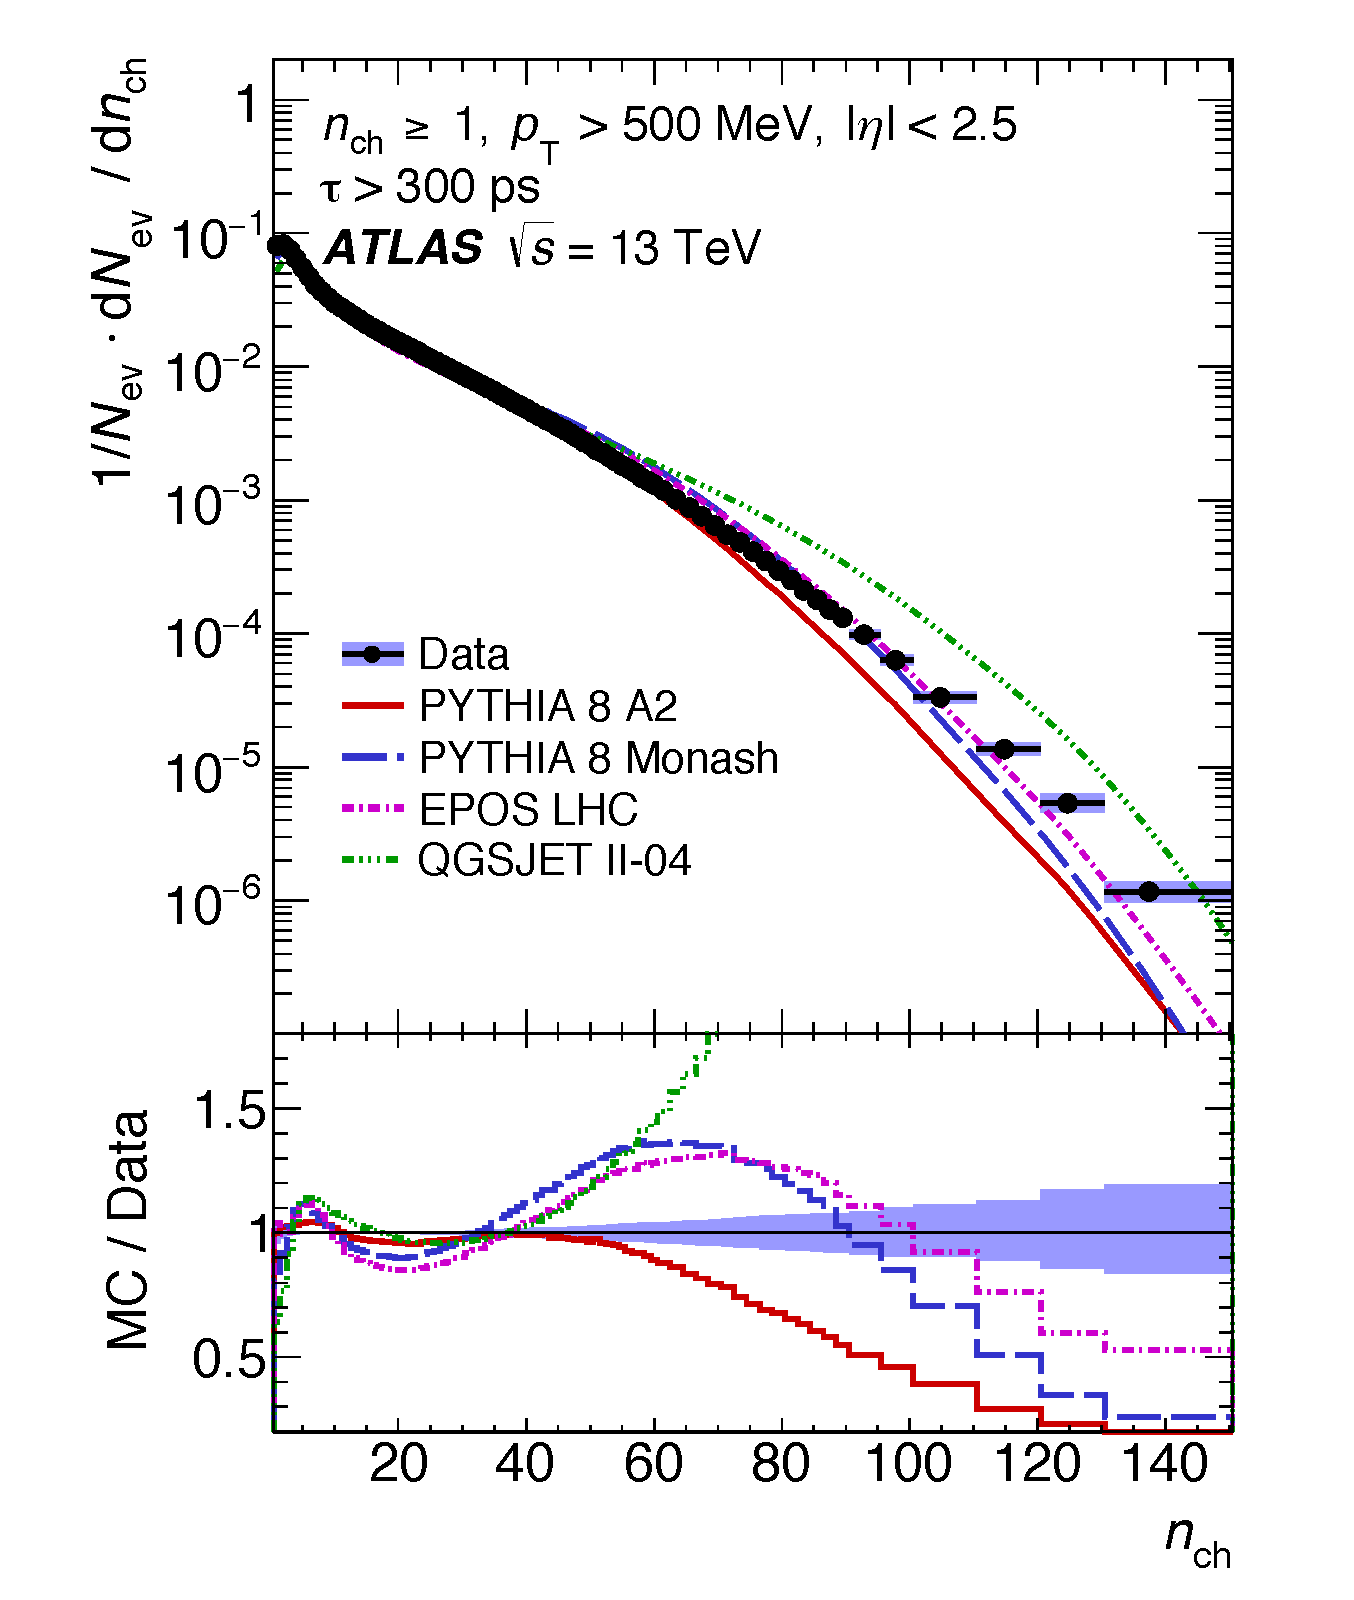
\includegraphics[width=.5\textwidth]{figures/DS_chargedParticleMultiplicities_pileup.pdf}
  \caption{Charged particle multiplicities measured in minimum bias events with the ATLAS detector for events with at least one track with a minimum \pt of 500~MeV and $|\eta|< 2.5$~\cite{Aad:2016mok}.}
  \label{fig:PILEUPchargedParticleMultiplicities}
\end{figure}

A major background to SUEP-like signals comes from pile-up, which also yields a large number of isotropically distributed soft tracks, though in contrast to SUEP signatures, stemming from multiple vertices. Studies on the multiplicity of charged tracks from minimum-bias interactions like single, double or non-diffractive collisions are described in~\cite{Aad:2016mok}. As shown in Fig.~\ref{fig:PILEUPchargedParticleMultiplicities}, the fraction of  13 TeV $pp$ collisions having 80 or more associated charged tracks is O($10^{-3}$), as measured in a pile-up-free environment.  Some benchmark SUEP models are described in~\cite{Knapen:2016hky} with a low-mass Higgs-mediator and two higher-mass scalar models, and charged particle multiplicities for these benchmarks are shown in Fig.~\ref{fig:SUEPchargedParticleMultiplicities}. (For those models only decays to electrons and muons were assumed.) Ref.~\cite{Knapen:2016hky} demonstrates that counting tracks associated to the PV should provide a very powerful discriminant against pile-up background during offline reconstruction for high mass mediators, while discrimination for the Higgs-mediator model is hardly possible. The crucial point for offline reconstruction is the number of particle tracks that can actually be reconstructed. Both ATLAS and CMS can reconstruct tracks with a minimum momentum of roughly 400~MeV~\cite{Sirunyan:2017ulk}. The multiplicity of tracks fulfilling this minimum-\pt requirement is shown in Fig.~\ref{fig:SUEPchargedParticleMultiplicities}c for the three SUEP benchmark models. Reconstructing hundreds of tracks could potentially become challenging when the tracks are not well-separated, but it was shown in~\cite{Knapen:2016hky} that even for the highest-mass mediator no significant losses of the tracking efficiency are expected. It is moreover worth noting that, while the track multiplicity is large compared to what is generated by SM proton-proton collisions, it is still relatively small compared to the multiplicities that can be reconstructed in heavy ion collisions. A large fraction of electrically neutral hadrons produced in the SUEP can further lower the number of associated tracks, which makes signal/background discrimination very difficult for the lowest-mass-mediator signals. A possible additional discriminant for those cases can be the hemisphere mass. This mass is estimated by dividing the event into a hemisphere associated to the ISR jet and one associated to the SUEP, while calculating the ``jet'' mass, as in Sec.~\ref{sec:darkshowerthinjet}, from the tracks in the SUEP hemisphere. This variable should be significantly higher for the SUEP events, where the heavy mediators are decaying, than for pile-up events.

\begin{figure}[tbp]
  \centering
  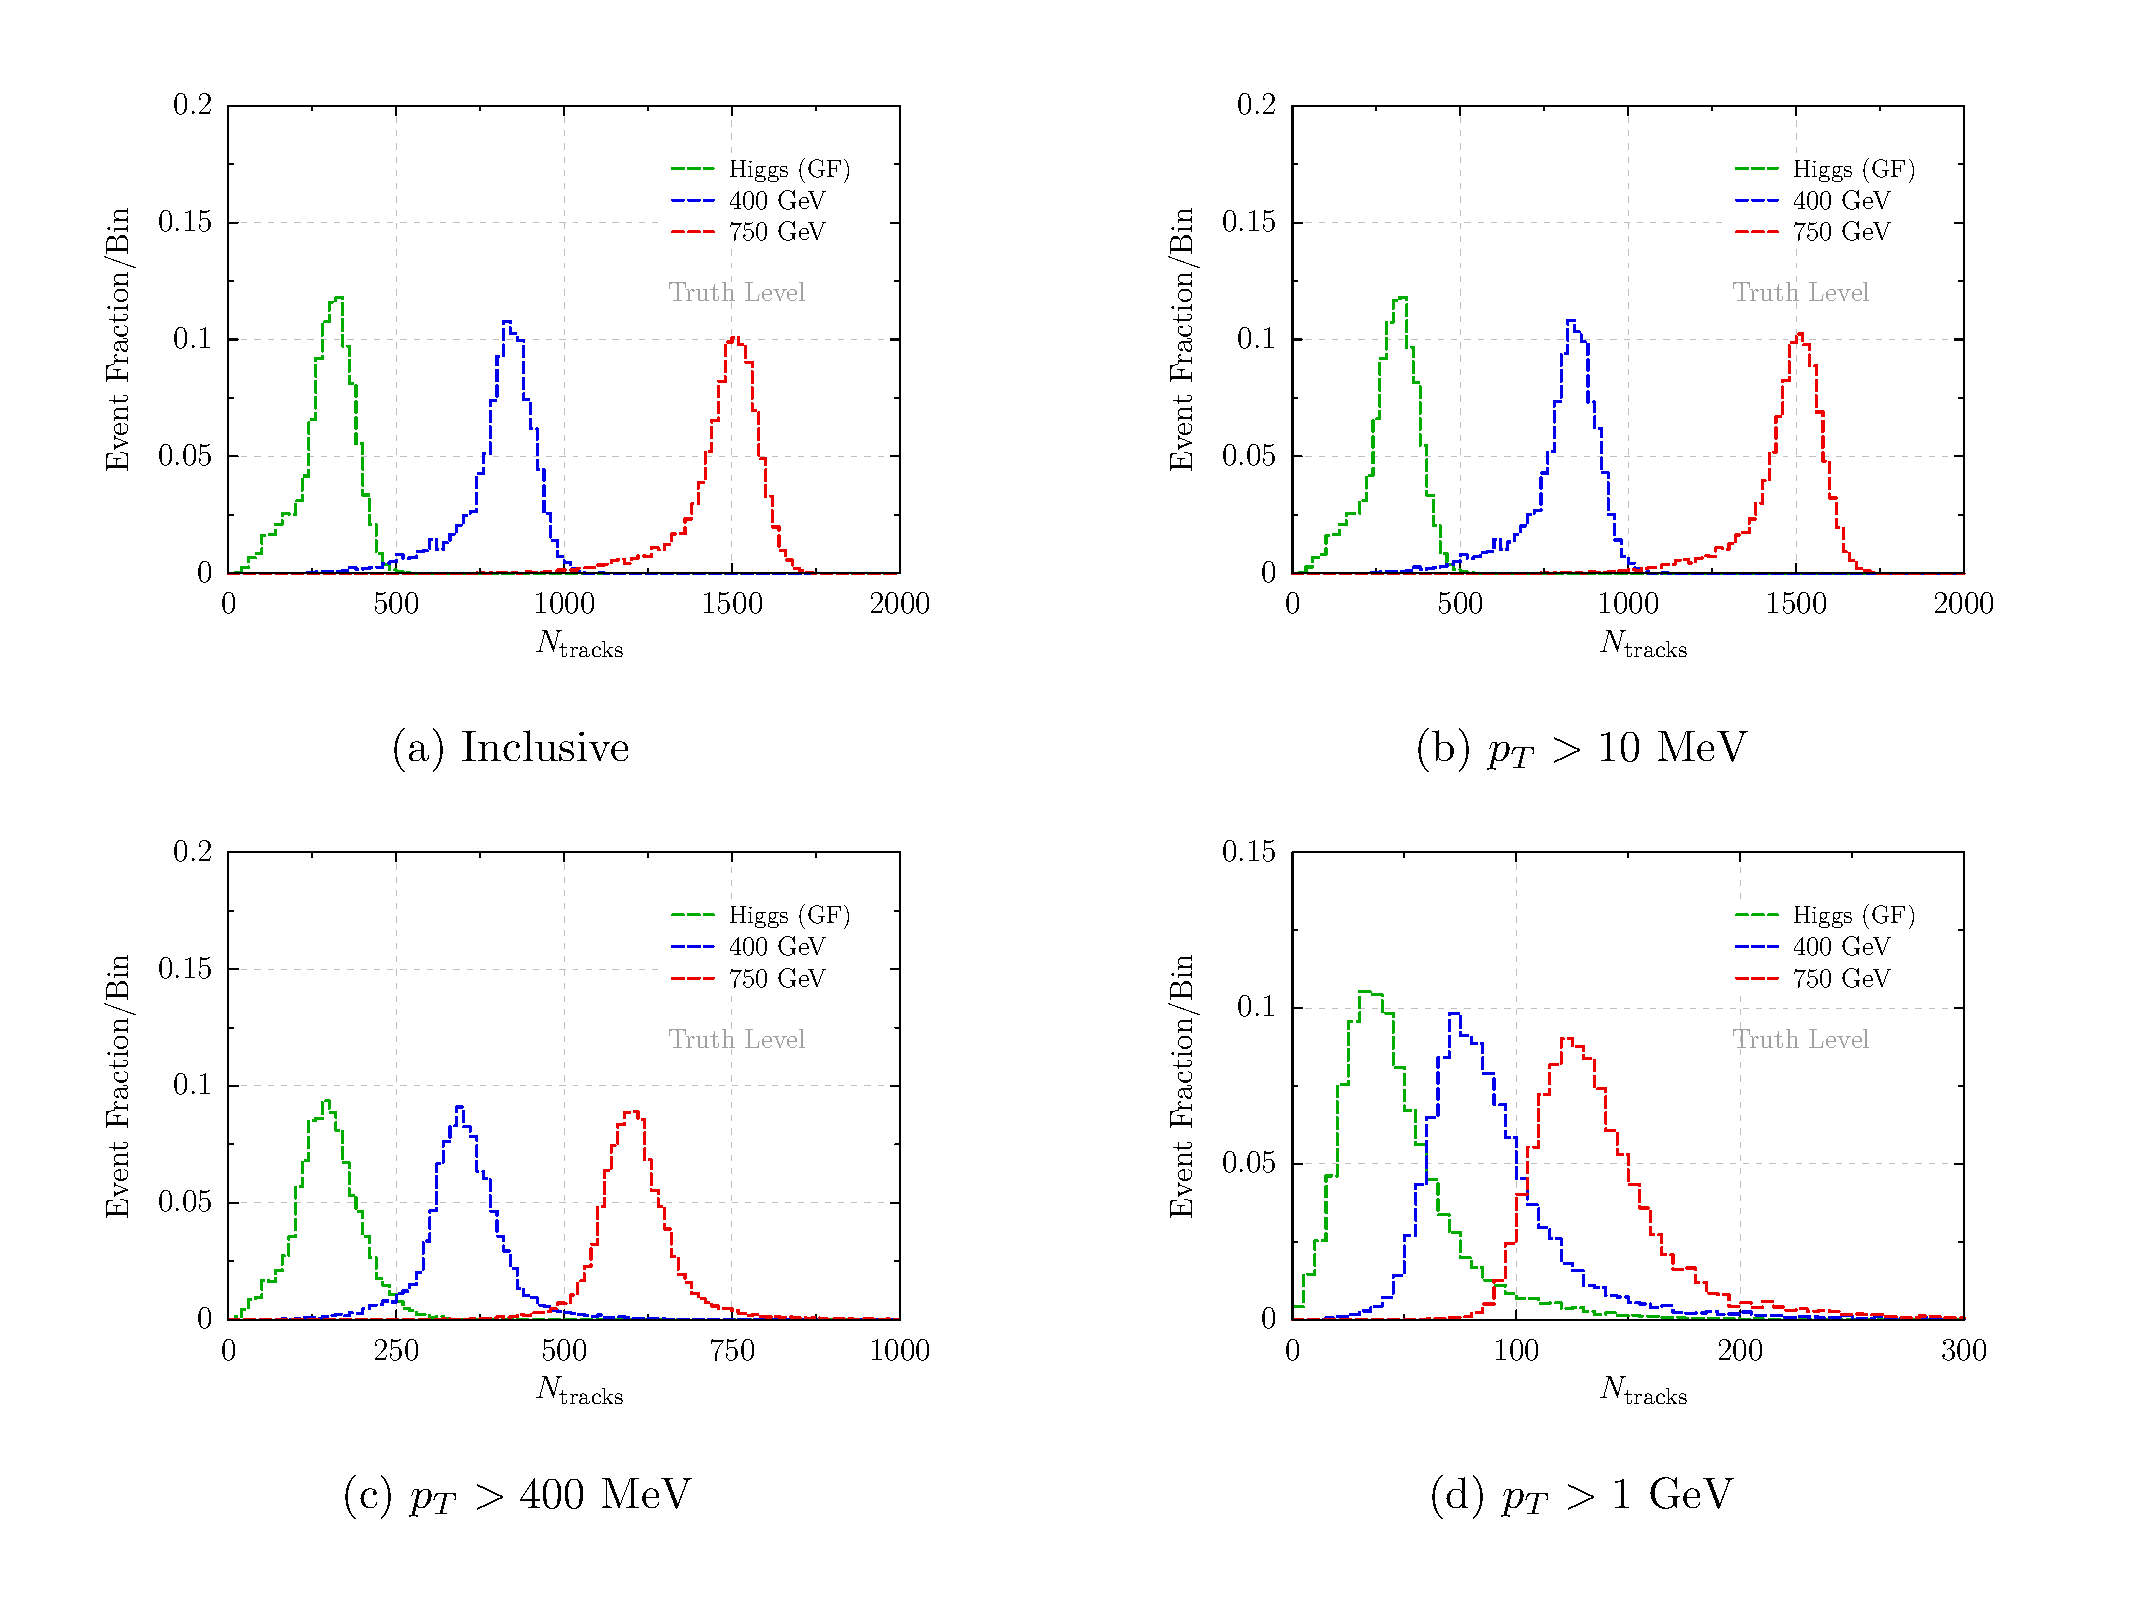
\includegraphics[width=.85\textwidth]{figures/DS_chargedParticleMultiplicities_SUEP.pdf}
  \caption{Event multiplicities of charged particle tracks fulfilling the respective indicated $p_{T}$ requirements for three benchmark SUEP models. Figure from Ref.~\cite{Knapen:2016hky}. }
  \label{fig:SUEPchargedParticleMultiplicities}
\end{figure}

Another possible background is QCD multi-jet events. Triggering SUEP events based on \MET relies, as described in Sec.~\ref{sec:darkshowertrigmultiplicity}, on the emission of an ISR jet recoiling against the system. QCD scenarios similar to SUEP signatures could arise when one hard jet is recoiling against a system of multiple soft jets. The mean number of charged tracks per jet is less than ten for jets $O(\text{100~GeV})$~\cite{Aad:2016oit}. To get to $O(100)$ charged tracks, as expected from a SUEP signature, a very high number of jets is needed, hence the perturbative cross section is heavily suppressed by many orders in $\alpha_{s}$. This background can nevertheless play a significant role for the low-mass mediator models, where significantly fewer tracks are expected. A veto against large calorimeter deposits can be a powerful handle to reject those events, as rather hard jets are needed to get many associated charged tracks.

\subsection{Displaced decays} % GREGOR
\label{sec:darkshowerdisp}

Outside the prompt regime, the lifetimes of the various dark states and the composition of SM final states produced in their decays drive the phenomenology. Specifically concerning the lifetime, the key question is whether there are one or more species of dark states in the hidden sector spectrum that would be stable in the absence of couplings to the SM. In particular different species naturally come with vastly different lifetimes, as is the case for the SM $\pi^0$ and $\pi^\pm$ mesons. In what follows, we consider the single species case in most detail, and treat the case of primarily leptonic decays (lepton-jets)  separately from the cases with substantial branching fractions to hadrons (emerging jets). We finally comment on the multi-species case, and relate it to the semi-visible jet scenario mentioned in the previous section. 

It is worth observing that even in high multiplicity events, the isolation of displaced decays from each other is not likely to pose difficulties in reconstructing DVs in the IT.  Two nearby DVs can be separately resolved down to separations of $\sim$ mm.  Even in the case where two DVs are closer than 1 mm, all of the tracks associated to both vertices will simply be reconstructed as a single DV with larger track multiplicity.  \JS{experimentalist eyes on this paragraph would be nice, as would suggestions for references}

\subsubsection{Single species leptonic dark showers (displaced lepton-jets)}
\label{sec:leptonjetsoffline}
One signature predicted by dark shower models is lepton-jets~\cite{Falkowski:2010cm,Falkowski:2010gv}, whose prompt decays are discussed in Sec.~\ref{sec:darkshowerprompt}. Depending on the lifetime of the decaying state, these leptons can easily be produced with a measurable displacement. Explicit searches for this signature  have been performed by the ATLAS collaboration at both 8 and 13 TeV~\cite{Aad:2014yea, ATLAS:2016jza}, as detailed in Sec.~\ref{subsec:dleptons}. It is worth remarking that the experimental signature of a displaced decay to electrons can be very similar to the signature of a displaced decay to a pair of charged pions, and thus searches for lepton jets frequently cover pionic final states as well.  Searches to date have targeted lepton-jets containing up to two lepton (pion) pairs.
%The existing searches already capture the most important features of a signal event. Yet, there is some information that
%are not yet taken into account or of which treatment can be improved. For instance, a dark shower model has typically missing energy that is aligned with the lepton-jet. This signature will be spurious in many case due to jet mis-reconstruction, however, if the mis-reconstruction can be quantified, for instance through a $Z\rightarrow jj$ control sample, it could still improve sensitivity.
%In addition, the particles emerging from a dark shower are usually close to the trigger threshold, thus one needs to stay as low in energy as possible, while instead exploiting the higher multiplicity.
To further extend coverage into low-mass regimes, it may be of interest here to investigate the samples stored through data scouting for e.g. di-muon resonances, although the limited information retained in scouted events likely makes this a promising avenue only for sufficiently short lifetimes that dedicated track reconstruction is not necessary.


\subsubsection{Single species hadronic dark showers (emerging jets)}
\label{sec:darkshoweremergingjets}


ATLAS, CMS, and LHCb have developed powerful searches for pairs of displaced vertices in the trackers, typically in association with missing energy or large $H_T$, as described in Sec.~\ref{subsec:djets}. These searches are nearly background-free and inclusive in the number of vertices, and thus have good sensitivity for any model of dark showers that has a large enough signal acceptance in such searches, regardless of the detailed features of the shower shape. 

While these searches demonstrate the power and flexibility of inclusive low-background searches, it is unfortunately very easy for signal acceptances in the existing displaced vertex searches to be prohibitively small.  Primary drivers for the loss of acceptance are the requirement of associated objects (leptons, MET, sizeable visible $H_T$, etc.), and/or cuts on the invariant mass of or number of tracks belonging to the displaced vertex. Given that a hidden shower tends to produce a multitude of vertices, it should be possible to maintain very low background levels---and therefore the power and inclusivity of the search---by relaxing many of these requirements and demanding a larger number of vertices instead.  In particular, it may be advantageous to bin signal and background in terms of the number of reconstructed vertices in a particular detector element with very loose $\eta$ and $\phi$ requirements, as well as transverse distance from the beampipe. This would allow for straightforward recasting to models with different shower shapes, lifetimes and $p_T$ spectra, allowing a single search to transparently apply to a very broad model space. If possible, it would also be useful to provide the distribution of background vertices as a function of the numbers of tracks, as this would help pin down decay modes, mass, etc.

When the lightest decaying dark state has mass $\lesssim 10$ GeV, backgrounds to DV searches do become more important, as the background DV rate rises rapidly as the number of tracks associated to the vertex falls; also, irreducible heavy-flavor backgrounds are important in this mass range. The number of associated tracks is also crucial for the vertex reconstruction in both the inner detector and the MS. Hence also the composition of hadronic and leptonic particles in the final states may have a significant impact on the ability to reconstruct the associated vertices and/or the size of the expected backgrounds. Moreover, as the track momentum and multiplicity in the vertices drop, the odds increase that one or more tracks belonging to a particular vertex are not reconstructed. If less than two tracks are reconstructed, clearly no vertex can be found, but a large number of unassociated tracks with a large impact parameter is still a striking signature. This is the idea behind a recent  CMS search \cite{CMS-PAS-EXO-18-001}, based on \cite{Schwaller:2015gea} (see below). Searches of this type are highly complementary with inclusive searches for multiple displaced vertices, as suggested above.
% We return to this case at the end of this subsection. 
Backgrounds also increase as the lifetime of the decaying dark state becomes shorter.  However even in this regime a dark shower offers many handles for signal/background discrimination beyond the number of vertices, such as a common mass scale for the vertices and non-SM-like particle multiplicity distributions.

 Given the striking nature of these high multiplicity signal events, it is typically not challenging to separate them from backgrounds once the event is on tape, provided that the DVs can be reconstructed. Frequently, reconstructing the DVs can require running dedicated re-tracking algorithms in order to identify highly displaced tracks. This re-tracking can be computationally expensive, and necessitates the preselection of at most $\sim 5\%$ of the total event sample on tape.  \JS{expert eyes on this paragraph are needed; also suggestions for refs  would be much appreciated}  In this case, the preselection criteria are likely to be the limiting factor in signal acceptance at the analysis level.

Dark showers produced through mediators carrying SM charges, such as the scenario of Ref.~\cite{Schwaller:2015gea}, generally provide ample preselection criteria through associated objects and relatively high overall event $H_T$ scales.  For instance, typical events for the model in Ref.~\cite{Schwaller:2015gea} contain two emerging jets and two QCD jets, though the additional two QCD jets can be absent in other models. The emerging jets can be reconstructed using default anti-$k_t$~\cite{Cacciari:2008gp} $R=0.4$ jets. A baseline preselection requires each jet to have $\pt > 200$~GeV, $\eta < 2.5$ and the scalar sum of jet \pt exceeding 1000~GeV. These criteria assume that jets can be reconstructed using the calorimeters which should be very efficient for the considered lifetimes. CMS has recently published a search for this model \cite{CMS-PAS-EXO-18-001},  where the search strategy hinges on the presence of a sizable number of high impact parameter tracks, without demanding a vertex. \cite{CMS-PAS-EXO-18-001} found excellent sensitivity for the benchmark model developed in~\cite{Schwaller:2015gea} and since it does not rely on vertex reconstruction, it is inherently very inclusive for models with a similar topology but a different hidden meson mass. A downside of this approach is that it is difficult to interpret this search in terms of other dark shower models as no vertex reconstruction was attempted. In this light we consider the track-based approach of Ref.~\cite{CMS-PAS-EXO-18-001} to be highly complementary with a vertex-based strategy. Ref.~\cite{CMS-PAS-EXO-18-001} is moreover an excellent demonstration that searches of this type are feasible despite the challenging nature of the signal.

When dark showers originate from a SM singlet, such as the Higgs boson or a $Z'$, the problem of preselection becomes more acute. The overall mass scale of signal events can easily be small, making event $H_T$ useless for signal separation.   Here perhaps one of the most robust avenues for preselection is muon multiplicity: as discussed in Sec.~\ref{sec:darkshowerdk}, many of the operators governing LLP decays tend to predict muon-rich final states.  With $\gg 2$ LLPs in an event, muon number becomes a useful and inclusive preselection criterion that places no demands on the possible presence of associated objects, event $H_T$, or detailed shower shape.  

For muon-poor low-mass dark shower events, pre-selection criteria become more model-dependent. When such dark showers originate from an exotic Higgs decay, SM Higgs production provides a suite of associated prompt objects that offer preselection handles, see Sec.~\ref{SM:secProduction_modes}, at some acceptance cost.   However it is also important to study to what extent features reflecting the presence of (multiple) LLPs in the event itself could be used as pre-selection criteria, e.g., anomalously track-poor jets, unusual ECAL/HCAL ratios (as realized by e.g. LLPs with $c\tau \lesssim$ m decaying dominantly to electrons and/or photons), anomalously large numbers of poorly reconstructed or high impact parameter tracks, etc.

Finally, the offline reconstruction for events where the vertices are low mass and/or very soft, as occurs in SUEP-style models, poses additional challenges. For the reconstruction of secondary vertices in the inner detector in ATLAS and CMS currently a minimum track \pt of 1~GeV is required \cite{Aaboud:2017iio,Chatrchyan:2012jua}. Having vertices with several tracks fulfilling this minimum \pt requirement might be rare if the hidden sector hadronization scale is low, in particular for the low mediator masses. In this case dedicated search strategies might be needed, especially for short lifetimes. For example, it may be possible to look for increased multiplicity of hits in the outer layers of the inner detector compared to the inner part, though unassociated hits from secondaries may be a significant background. Potentially a subtraction of hits from tracks stemming from vertices close to the beam pipe might be helpful, but dedicated studies are needed to assess the viability of this approach.
In addition, the calorimeter may be another handle on this type of events: a large collection of soft particles could collectively contribute an interesting energy pattern in the calorimeters, if the lifetime is long enough and if the segmentation in radial direction is exploited. However, if the hidden mesons can reach the calorimeter, their decays typically takes place over a distance longer or comparable to the size of the calorimeter itself. This effect could wash out the signal to the extent that it may be difficult to observe above background, though a full truth-level simulation of this effect is certainly warranted.
 




\subsubsection{Multi-species dark showers \label{sec:darkshowersemivisible}}

If there are multiple species in the dark shower that decay to SM final states, the lifetimes of these species will in general be very different. The intermediate case where most mesons decay with a macroscopic lifetime produces similar phenomenology to the single-species models discussed above. Another regime occurs when at least one species decays promptly, while the others are either stable or decay outside of the detector, which gives rise to a semi-visible jet~\cite{Cohen:2015toa} (Sec.~\ref{sec:darkshowerthinjet} above).  The intermediate scenario, where some dark states decay promptly while others have macroscopic detector-scale lifetimes, is equally generic. A combination of semi-visible techniques with displaced vertex reconstruction can be used to boost sensitivity in this case.  As for the discussion above, it is important here to pay attention to potential isolation criteria on DVs, as the presence of potentially large numbers of promptly-decaying dark particles may necessitate their relaxation.

\section{Executive Summary}
\label{sec:darkshowersummary}

Dark showers are a common prediction of a wide range of hidden sector theories. % which present a vast model space with many areas of theoretical uncertainty.  
Although the model space is dauntingly enormous, it is possible to make some very general statements about the {\em signature} space of interest: dark shower events can be characterized by (1)  a variable and frequently large multiplicity of particles per event; (2) BSM states with a hierarchy of proper lifetimes, making the existence of at least one LLP species generic; (3)  frequently, non-isolation of LLPs from other objects in the event; and (4) non-SM-like energy flow and particle multiplicity.   These features typically ensure that dark shower events will be very distinctive signatures in the generic regime where at least one species has a detector-scale lifetime.  Thus it should be possible to design powerful and inclusive searches which would be sensitive to a very large portion of the vast model space without needing to rely on poorly predicted (and model-dependent) properties such as shower shape.   Toward this end we have identified several promising directions for future study for both theory and experiment, and provide some recommendations here.

As always, one of the primary challenges in searches for dark showers is ensuring the events are recorded on tape.  In some models, dark showers may be accompanied by a decent amount of MET or $H_T$, or associated leptons, but it is important to remember that there are many scenarios where this is not the case, or where these handles come at the expense of a large reduction in signal rate. The foremost example of this is when the dark shower is initiated by an exotic Higgs decay.  It is thus critical to pursue dedicated trigger strategies, and we present a few ideas here. We expect that displaced triggers designed for singly- or doubly-produced LLPs will typically have reasonable acceptance for dark shower events, though we caution that in some cases the non-isolation of LLPs in dark shower events may limit their acceptance.  Another promising avenue for triggering on dark showers exploits the high particle multiplicity typical of such events, and we recommend study of triggers on (displaced) multi-muons in particular.  

The off-line analysis of dark shower events poses several challenges as well.  At this time, only the limiting cases of pencil-like or fully spherical showers are under good theoretical control.  New studies of showering in the intermediate regime were performed for the purpose of this white paper (Sec.~\ref{sec:darkshowershower}), which revealed that different approaches can yield qualitatively different phenomenology.  On one hand this provides interesting opportunities for searches which make use of event shape and/or jet substructure variables, in particular if the decay of the hidden sector states occurs promptly or with small displacements. On the other hand, for larger displacements it implies that one should be careful not to heavily bias the selection choices of a search towards a particular shower shape, and rely instead on the displaced LLP decays to separate signal from background.  We expect that the most inclusive, most broadly applicable, and most recastable searches would be those where the data is binned in terms of the number of reconstructed vertices and their  location within the detector.  For recasting purposes, and to assist with unraveling the underlying physics in the event of a discovery, it would moreover be important to supply information concerning distributions of the number of tracks per vertex and/or the vertex mass whenever possible.

The presence of $N_{DV}\gg 2$ displaced vertices in an event will be enormously powerful for background suppression, provided those vertices can in fact be reconstructed. To identify highly displaced tracks, it may be necessary to run dedicated and  computationally expensive re-tracking algorithms,  requiring the imposition of some preselection criteria to identify events of interest.   As these preselection criteria are likely to be the limiting factor controlling post-trigger signal acceptance in many models, we recommend developing criteria for dark showers that rely on particle multiplicity and, if possible,  the presence of multiple LLPs in the event, while keeping $p_T$ thresholds as low as possible.  \\

\vspace{1cm}
\textbf{Acknowledgments}\\
We thank Laura Jeanty, Ted Kolberg, Simone Pagan Griso, Brian Shuve, ... for useful discussions.

\section{Appendix:~Example models}
\label{sec:darkshowermodels}
In this appendix we survey the models for which currently Monte Carlo is available. 

\subsection{Lepton Jets from Radiating Dark Matter }


%At the partonic center of mass energies afforded by the LHC, radiative processes
%have reached unprecedented levels. They are omnipresent not only
%in QCD and electroweak interactions, but will also appear in dark sectors that
%contain light new particles with sizeable couplings.  This applies in particular
%to models of self-interacting dark matter~\cite{Spergel:1999mh,
%Tulin:2013teo}, which could potentially resolve shortcomings of our present
%understanding of cosmic structure formation on dwarf galaxy scales (see also
%\cite{Vogelsberger:2014kha, Sawala:2014xka}).  Such dark sectors can also
%feature Sommerfeld enhancement in DM annihilation \cite{Hisano:2003ec,
%Cirelli:2008pk, ArkaniHamed:2008qn}, and may even lead to to the formation of DM
%bound states \cite{Shepherd:2009sa, Altmannshofer:2014cla}.

One of the simplest and most widely discussed types of light dark sector particle is a
dark photon $A'$, i.e.\ a new gauge boson associated with a local $U(1)$
symmetry in the dark sector.  By kinetically mixing with the SM photon, a dark
photon can act as the mediator of dark matter--SM interactions, in addition to being
responsible for DM self-interactions.  Phenomenologically most relevant are
dark photons in the mass range between MeV and GeV.  The dark sector Lagrangian
in such a scenario reads
\begin{align}
  \mathcal{L}_\text{dark} \equiv
  \bar{\chi} (i\slashed{\partial} - m_\chi + i g_{A'} \slashed{A'}) \chi
    - \frac{1}{4} F'_{\mu\nu} F'^{\mu\nu}
    + \frac{1}{2} m_{A'}^2 A'_\mu A'^\mu
    - \frac{\epsilon}{2} F'_{\mu\nu} F^{\mu\nu} \,.
  \label{eq:L-radiating-DM}
\end{align}
Here, $\chi$ is the fermionic DM particle with mass $m_\chi$, and $g_{A'} =
\sqrt{4 \pi \alpha'}$ is the $U(1)'$ gauge coupling. From the point of view of dark showers, interesting values for the
strength are $\alpha' \gtrsim 0.01$. If $\alpha'$ is much smaller, there
is too little radiation to form a dark shower.  The dark photon mass is denoted by
$m_{A'}$, and the kinetic mixing parameter by $\epsilon$. Typically, $\epsilon$
is required to be $< 10^{-3}$.  We remain agnostic about the origin of the dark
photon mass---it could originate from a dark sector Higgs mechanism or from the
St\"uckelberg mechanism.

If $m_\chi \ll 100$~GeV, DM particles may be produced at the LHC with a large
boost.  This entails a large probability for radiating additional collinear
$A'$ bosons (see fig.~\ref{fig:radiating-dm-diagram}).  A detailed analytical
and numerical description of such dark photon showers has been presented in
ref.~\cite{Buschmann:2015awa}. The $A'$ bosons eventually decay to
observable SM particles through the kinetic mixing term in
eq.~\eqref{eq:L-radiating-DM}.
Depending on the value of $\epsilon$, the decays can be either prompt or
displaced. Phenomenologically, the final state of the process $p p \to \bar\chi
\chi + n A'$ thus consists of two ``jets'' of collimated $A'$ decay products,
plus missing energy.

\begin{figure}[b]
  \begin{center}
    \includegraphics[width=0.4\textwidth]{figures/DS_darkradiation.pdf}
  \end{center}
  \vspace{-0.7cm}
  \caption{The process that gives radiating dark matter its name: production of
    two DM particles $\chi$, followed by the emission of several soft or collinear
    dark photons $A'$~\cite{Buschmann:2015awa}.}
  \label{fig:radiating-dm-diagram}
\end{figure}

\begin{figure}
  \begin{center}
    \includegraphics[width=0.95\textwidth]{figures/DS_DarkPhoton_BR.pdf}
  \end{center}
  \vspace{-0.7cm}
  \caption{Branching ratios of a kinetically mixed dark photon $A'$as a
    function of $m_{A'}$~\cite{Buschmann:2015awa}.}
%    The computation was carried out in Pythia~8~\cite{Carloni:2010tw,
%    Carloni:2011kk, Sjostrand:2014zea}, using the hidden valley model implemented
%    therein. See ref.~\cite{Buschmann:2015awa} for an analytic treatment
%    of dark radiation.}
  \label{fig:radiating-dm-BR}
\end{figure}

The $A'$ branching ratios into different SM final states depend sensitively on
$m_{A'}$ (see fig.~\ref{fig:radiating-dm-BR}).  At $m_{A'} \lesssim 400$~MeV, the dominant
decay modes are $A' \to e^+e^-$ and $A' \to \mu^+ \mu^-$. The decay
rate into each lepton flavor $\ell$ is
\begin{align}
  \Gamma(A' \to \ell^+\ell^-) =
    \frac{1}{3} \alpha \epsilon^2 m_{A'}
    = \frac{1}{8 \times 10^{-6}\,\text{cm}}
      \bigg( \frac{\epsilon}{10^{-3}} \bigg)^2
      \bigg( \frac{m_{A'}}{\text{GeV}} \bigg) \,,
\end{align}
where $m_\ell \ll m_{A'}$ has been assumed for simplicity.
For purely leptonic decays, the $A'$ shower thus corresponds to a ``lepton
jet'', i.e.\ a set of collimated leptons. This signature has been
previously discussed for instance in refs.~\cite{ArkaniHamed:2008qp,
Cheung:2009su, Katz:2009qq, Bai:2009it, Baumgart:2009tn, Chan:2011aa,
Falkowski:2010gv, Curtin:2013fra, Gupta:2015lfa, Autran:2015mfa}.
Experimental searches for lepton jets have been presented in
refs.~\cite{Aad:2014yea, Aad:2015sms, ATLAS:2016jza, Khachatryan:2015wka},
where refs.~\cite{Aad:2014yea, ATLAS:2016jza} focus on lepton jets with
displaced vertices.

Lepton jet searches may also be sensitive to dark photons
with masses $\gtrsim 400$~MeV, even though the leptonic branching ratio is reduced
to between 20\% and 70\% in this regime. The mix of leptons and hadrons
expected from $A'$ decays at $m_{A'} \gtrsim 400$~MeV implies, however,
that most leptons will not be isolated, but occur in conjunction with hadronic
activity in the same detector region.  In view of this, dedicated trigger and
analysis strategies may significantly boost the sensitivity (see Sec.~\ref{sec:leptonjetsoffline}). 

In certain parameter regions, the decays of radiated $A'$ bosons may closely
resemble a purely hadronic QCD jet. This will happen in particular when $m_{A'}$
is close to a QCD resonance, or when the average $A'$ multiplicity in each
shower is low, and the hadronic branching ratio is sizeable. In this case,
separation of the signal from the QCD background will most likely be possible
only if $\epsilon$ is so small that $A'$ decays are displaced.

Let us summarize several important considerations to take into account when
devising a search for dark sector radiation:
\begin{itemize}
  \item {\bf There may or may not be a signal in the tracking detector.}
    Prompt $A'$ decays will typically lead to such signals, except for specific
    $A'$ decay modes to neutral particles, for instance $A' \to K^0 \bar{K}^0$
    and $A' \to \pi^0 \gamma$. Displaced $A'$ decays can also leave a signal in the tracker, 
    however if the lifetime is sufficiently long more decays will occur in the muon chamber (see Sec.~\ref{sec:darkshowerctau}). 

  \item {\bf There may or may not be a signal in the calorimeters.} Most $A'$
    decay modes will be visible to the calorimeters (with the exception of $A'
    \to \mu^+ \mu^-$). However, it is important to realize that a signal in the
    hadronic calorimeter can arise not only from hadronic activity, but also
    from displaced decays to lepton occuring inside the calorimeter.
  
  \item {\bf There will be missing energy contained within the lepton jet.}
    As the decaying $A'$ bosons are aligned with the DM particle from which
    they were radiated, the corresponding missing momentum vector points in
    the same direction. However, unless there is significant initial
    state radiation, the missing momentum will typically be balanced between
    the two showers shown in fig.~\ref{fig:radiating-dm-diagram}, and
    will therefore not be detectable experimentally. 
\end{itemize}

In fig.~\ref{fig:radiating-dm-limits}, we show for
illustration the exclusion limits that past LHC searches place on the dark photon
parameters.

\begin{figure}
  \begin{center}
    \includegraphics[width=0.6\textwidth]{figures/DS_DarkPhoton_Constraints.pdf}
  \end{center}
  \vspace{-0.7cm}
  \caption{
    95\% CL constraints on the dark photon mass $m_{A'}$ and the kinetic mixing
    parameter $\epsilon$, for $m_\chi = 4$~GeV, $\alpha_{A'} = 0.2$.  We have
    assumed $\chi$ production through a $Z'$ portal with mass 1 TeV, with a production cross
    section of 0.58~pb at $\sqrt{s} = 7$~TeV and 0.85~pb at 8~TeV.
    We show exclusion limits from the ATLAS search for prompt lepton
    jets in 5~fb$^{-1}$ of 7~TeV data~\cite{Aad:2012qua} (blue shaded region)
    and from their displaced lepton jet search in 20.3~fb$^{-1}$ of 8~TeV
    data~\cite{Aad:2014yea} (red shaded region).
    The lighter colored region around $m_{A'}=2$ GeV corresponds to the
    transition region between an analysis in terms of hadron final states and
    an analysis in terms of quark final states and is based on interpolation.
    The computation was carried out in Pythia~8~\cite{Carloni:2010tw,
    Carloni:2011kk, Sjostrand:2014zea}, see \cite{Buschmann:2015awa} for
    details.  We also show the existing 90\% CL exclusion limits from the
    electron and muon anomalous magnetic
    moment~\cite{Pospelov:2008zw,Davoudiasl:2012ig,Endo:2012hp},
    HADES~\cite{Agakishiev:2013fwl}, KLOE 2013~\cite{Babusci:2012cr} and
    2014~\cite{Babusci:2014sta}, the test run results from
    APEX~\cite{Abrahamyan:2011gv}, BaBar 2009~\cite{Aubert:2009cp} and
    2014~\cite{Lees:2014xha}, beam dump experiments E137, E141, and
    E774~\cite{Blumlein:2011mv,Bjorken:2009mm,Bross:1989mp},
    A1~\cite{Merkel:2011ze}, Orsay~\cite{Davier:1989wz},
    U70~\cite{Blumlein:2013cua}, CHARM~\cite{Gninenko:2012eq},
    LSND~\cite{Essig:2010gu}, as well as constraints from astrophysical
    observations~\cite{Dent:2012mx,Dreiner:2013mua} and $\pi^0$
    decays~\cite{CERNNA48/2:2015lha}. Figure based on
    ref.~\cite{Buschmann:2015awa}.}
  \label{fig:radiating-dm-limits}
\end{figure}





\subsection{Emerging jets and semi-visible jets from a heavy colored mediator}


Hidden valley models~\cite{Strassler:2006im} with QCD-like hidden sectors allow for interesting collider signatures. Thus we consider a confined dark gauge group SU($N_{d}$), where $N_{d} \geq 2$, with confinement scale $\Lambda_{d}$ which sets the mass of the dark hadrons. There are also $n_f$ flavors of dark quarks whose bare masses are lighter than $\Lambda_d$. The hidden valley comes equipped with a portal that couples the dark sector to the SM, and the mass is usually taken to be $M \gg \Lambda_d$. The portal can be an $s$-channel vector mediator, $Z_d$ which couples to SM quarks and dark quarks:
\begin{equation}
\mathcal{L} \supset - Z_{d,\mu} \sum_{i,a} \big( g_q \, \overline{q}_i\gamma^\mu q_i + g_{q_{d}} \, \overline{q}_{d,a} \gamma^\mu q_{d,a}  \big) \, ,
\label{eq:schannelL}
\end{equation}
where $g_{q/q_{d}}$ are coupling constants and $i,a$ are flavor indices.  One can also have a $t$ channel scalar bifundamental mediator, $X$, which carries color and dark color and can decay to a quark and a dark quark. In the case of the scalar mediator, the only allowable coupling is of the form
\begin{align}
	{\cal L} \supset \kappa_{ij} \bar{q}_i q_{d,j} X + {\rm h.c.}\,,
	\label{eqn:yukawacoupling}
\end{align} 
where, $\kappa_{ij}$ is a $3\times n_f$ matrix of Yukawa couplings. One could also add multiple flavors of $X$ mediators, something that has also been implemented.
%\vspace{1em}

When dark quarks are produced, they shower and hadronize and we can use the same tools that are familiar for QCD to simulate these processes. Because of the large gap between the mediator mass and the confining scale, there will be large particle multiplicity and the dark hadrons will typically form into jet-like structures. In the large $N_{d}$ limit, the fraction of dark baryons produced is suppressed, and in the case of QCD this fraction is $\mathcal{O}(0.1)$. Therefore the simulations typically have the dark mesons to dominate hadronization. The lightest hadronic states are the dark pions $\pi_{d}$, acting as goldstone bosons of the $U(n_{f}) \times U(n_{f})$ dark flavor symmetry. When a heavier mesonic state is produced it will promptly decay into dark pions if kinematically allowed, making the dark pions the dominant component of the dark showering process. 

%\vspace{1em}

We can simulate these events with the Hidden Valley~\cite{Carloni:2010tw} version of \verb!Pythia8!~\cite{Sjostrand:2014zea}. \verb!Pythia8! hosts a hidden valley class which incorporates the $SU(N_{d})$ model, allowing the user to vary the masses of the spectrum ($\pi_{d}, \rho_{d}, etc$), number of flavors $n_{f}$, and parameters of the running coupling (Version $\geq$ 8.226). Pair production of $X$ and resonant production of $Z_d$ are implemented at tree level, and there is also decay of dark mesons to SM states.

In both~\cite{Cohen:2017pzm,Linthorne:2018abc}, production of the heavy mediators with ISR/FSR was considered. This was done by interfacing with \verb!Madgraph5_aMC@NLO!~\cite{Alwall:2014hca} using a modified version of the spin-1 \texttt{DMsimp} model\footnote{\url{http://feynrules.irmp.ucl.ac.be/wiki/DMsimp}} implemented through \texttt{FeynRules}~\cite{Alloul:2013bka}.
The models are located in the repository\footnote{\url{https://github.com/smsharma/SemivisibleJets}} folder \texttt{DMsimp\_s\_spin1}.  The generation files for the t-channel exchange of the scalar $X$  are located in the folder \texttt{DMsimp\_tchannel}. The bi-fundamentals are denoted with \texttt{su11, su12, su21, su22}\ldots, where \texttt{u} explicitly specifies the QCD flavor index and the numbers are the explicit dark non-Abelian group indices. Similarly, the dark quarks are labeled as \texttt{qv11, qv12, qv21, qv22}. A \texttt{FeynRules} model file (\texttt{DMsimp\_tchannel.fr}) as well as the Mathematica notebook (\texttt{DMsimp\_tchannel.nb}) used to generated the UFO output are also provided. The showering and hadronization in the dark sector can still be performed in \verb!Pythia8!. 

%Jets can be clustered using the same anti-$k_{T}$ algorithm as is used for QCD jets.

\subsubsection{Semi-visible Jets}

Generically, some of the dark pions could decay promptly and some could be long-lived or even collider stable, analogous to the neutral vs.~charged pions in the SM. If both stable and unstable hadrons are produced in a collision, the missing energy could be aligned along one of the jets, resulting in low acceptance for traditional monojet-style searches. This is the semi-visible jets scenario, and Refs.~\cite{Cohen:2015toa,Cohen:2017pzm} introduce a Simplified Model-like parameterization to map the complicated dynamics of the underlying dark sector onto a limited number of physically-motivated variables---in particular, the fraction of stable vs decaying pions, the characteristic mass scale of dark pions and the dark coupling strength. The Monte Carlo production described here along with the \texttt{Pythia8} Hidden Valley module allows the user to vary these parameters for the $s$- and $t$-channel UV completions. See Refs.~\cite{Cohen:2015toa,Cohen:2017pzm} for further details.

\subsubsection{Emerging Jets}
One can also take all the pions to have detector scale lifetimes, this is the emerging jets scenario~\cite{Schwaller:2015gea}. One can quantify the expected lifetime of the dark pions using Eq.~\ref{eqn:yukawacoupling}.  Under the assumption of universal couplings 
$\kappa_{ij} = \kappa$ and $m_{q} > \Lambda_{d}$, we can calculate the proper lifetime of the dark pions:
%
\begin{align}
	c \tau_{0} \approx 80 \mathrm{mm} \times \frac{1}{\kappa} \times \left( \frac{2 \;\mathrm{GeV}}{f_{\pi_{d}}} \right)^2 \left( \frac{100 \;\mathrm{MeV}}{m_{q}} \right) \left( \frac{2\; \mathrm{GeV}}{m_{\pi_{d} }} \right) \left( \frac{M_{X}}{1 \;\mathrm{TeV}} \right)^4 \,,
\end{align} 
where, $f_{\pi_{d}}$ is the dark pion decay constant, and $m_q$ is the mass of the SM quark in the final state.  A similar formula comes out for the $Z_d$ mediator. Therefore a jet of dark hadrons will be created as dominantly invisible particles, but at long distance, the dark pions will decay back to Standard Model particles and appear like an ordinary jet. The jet emerges as it travels through the detectors.

%\vspace{1em}

In the case of purely $t$-channel interactions, having a non-trivial $\kappa_{ij}$ in Eq. (1) will break the $U(n_{f}) \times U(n_{f})$ dark flavor symmetry. With an appropriate $n_{f}$ the dark quark flavors can be exactly aligned with the SM down quark flavors. It is immediately clear that such alignment leads to dark pions with lifetimes that differ significantly
from one another. In return, the flavor composition of the emerging jets will vary throughout the detector volume. This differs from the $s$-channel interaction, in which, no breaking occurs and $n_{f}$-stable vs. $n_{f}(n_{f} - 1)$-unstable dark pions exist. 

\subsection{SUEPs}
In the strongly coupled regime, dark showers can be become spherical and almost arbitrarily soft. In this case the sheer multiplicity of the final states becomes the most important experimental handle. It has been shown through the AdS/CFT correspondence that their spectrum should follow an approximately thermal distribution \cite{Hatta:2008qx}, which is what was assumed in the phenomenological study in~\cite{Knapen:2016hky}. The production mechanism for these studies was the Higgs or a heavy Higgs-like scalar. The Monte Carlo code that was written for this study is currently not available publicly, though events in hepmc format can be obtained by contacting the authors. At this time only leptonic decays of the hidden mesons are implemented.  




